\documentclass[inzynier,druk]{dyplom}
\usepackage[utf8]{inputenc}
\usepackage{hyperref}
\usepackage{booktabs}
%%
\usepackage[toc]{appendix}
\renewcommand{\appendixtocname}{Dodatki}
\renewcommand{\appendixpagename}{Dodatki}

% pakiet do sk?adu listing?w w razie potrzeby mo?na odblokowa? mo?liwo?? numerowania linii lub zmieni? wielko?? czcionki w listingu
\usepackage{minted}
\setminted{breaklines,
frame=lines,
framesep=5mm,
baselinestretch=1.1,
fontsize=\small,
%linenos
}

% nowe otoczenie do składania listingów
\usepackage{float}
\newfloat{listing}{htp}{lop}
\floatname{listing}{Listing}
\let\counterwithout\relax
\let\counterwithin\relax
\usepackage{chngcntr}
\counterwithin{listing}{chapter}

% patch wyr?wnuj?cy spis listing?w do lewego marginesu
%https://tex.stackexchange.com/questions/58469/why-are-listof-and-listoffigures-styled-differently
\makeatletter
\renewcommand*{\listof}[2]{%
  \@ifundefined{ext@#1}{\float@error{#1}}{%
  \expandafter\let\csname l@#1\endcsname \l@figure% <- use layout of figure
    \float@listhead{#2}%
    \begingroup
      \setlength\parskip{0pt plus 1pt}%               % <- or drop this line completely
        \@starttoc{\@nameuse{ext@#1}}%
    \endgroup}}
\makeatother

\usepackage{url}
\usepackage{lipsum}

% Dane o pracy
\author{Karol Kowalski}
\title{Aplikacja wspomagająca zdalne szacowanie historyjek użytkownika metodą
Planistycznego Pokera}
\titlen{Application supporting remote user stories estimation
using Planning Poker method.}
\promotor{dr. \ hab. \ inż. \ prof. PWr. Trawiński Bogdan}
%\konsultant{dr hab. in?. Kazimerz Kabacki}
\wydzial{Wydział Informatyki i Zarządzania}
\kierunek{Informatyka}
\krotkiestreszczenie{Praca przedstawia analizę problemu estymacji zadań
w projektach prowadzonych metodykami zwinnymi. Zawiera opis projektu aplikacji
umożliwiającej przeprowadzenie rozgrywki planning pokera online,
stworzonej przy użyciu nowoczesnych narzędzi webowych: ReactJS i Firebase.}
\slowakluczowe{metodyki zwinne, estymacja zadań, historyjki użytkownika, planning poker}

\begin{document}

\maketitle

\tableofcontents

\listoffigures

\listof{listing}{Spis listingów}

\listoftables

% --- Strona ze streszczeniem i abstraktem ------------------------------------------------------------------
\chapter*{Streszczenie} % po polsku
Niniejsza praca zawiera omówienie wybranych metod zwinnych zarządzania projektami,
ze szczególnym uwzględnienie technik wykorzystywanych
do estymacji zadań projektowych w tych metodykach.
Spośród znanych autorowi technik, najbardziej rozpowszechnioną jest tzw. Planning Poker.
Można znaleźć wiele aplikacji wspomagających proces estymacji przy wykorzystaniu
tej techniki, jednakże autor nie znalazł wśród nich żadnej, która pozwalałaby
na integrację z popularnym narzędziem Github.

Celem pracy było zaprojektowanie oraz wykonanie aplikacji wspomagającej grę
Planning Poker. Jej potencjalnymi użytkownikami są zespoły programistów
pracujących w trybie zdalnym, które wykorzystują narzędzie Github w codziennej pracy.

W ramach pracy autor stworzył aplikację typu Single-page opartą o architekturę Flux
oraz wykorzystującą usługę Firebase jako tzw backend.
Wyróżniającą cechą aplikacji jest możliwość importu historyjek
(tzw issues) z Githuba oraz zapisu rezultatów sesji planingowych za pomocą
odpowiedniego etykietowania historyjek w Github.

Użyteczność aplikacji została zweryfikowana w oparciu o wyniki ankiety,
które zostały zawarte w niniejszej pracy.


% Kilka sztuczek, ?eby:
% - Abstract pojawi? si? na tej samej stronie co Streszczenie
% - Abstract nie pojawi? si? w spisie tre?ci
\addtocontents{toc}{\protect\setcounter{tocdepth}{-1}}
\begingroup
\renewcommand{\cleardoublepage}{}
\renewcommand{\clearpage}{}
\chapter*{Abstract} % ...i to samo po angielsku
The thesis describes a few agile project management methods with the emphasis
put on techniques used for user stories estimation.
The well-established technique is Planning Poker.
There are many application that support this technique, although the thesis
author could not find a one that would offer any kind of integration with
Github.

The main goal of this thesis was to design and develop a web application to play
Planning Poker online. The target of the application are remote teams of software
developers that use Github in everyday work.

The created application is a Single-page app based on Flux architecture
that uses Firebase service for backend.
The \textit{killer feature} of the application is the integration with
Github that allows to import and filter issues and save the results of
estimation sessions as issue labels.

The usability of application has been verified based on a survey given to
application users. The survey results are included in the thesis.
\endgroup
\addtocontents{toc}{\protect\setcounter{tocdepth}{2}}
% --- Koniec strony ze streszczeniem i abstraktem -----------------------------------------------------------



% Rozdzia? do??czony z zewn?trz
\chapter*{Wstęp}
Planowanie to odpowiadanie na pytanie „Co powinniśmy stworzyć i kiedy?”.
Jednak aby odpowiedzieć na to pytanie powinniśmy zadać również pytania o estymację
(„Jak duże to jest?”) oraz harmonogram („Kiedy będzie skończone\text{?}” oraz „Ile będzie zrobione do tego czasu?”).
Estymowanie i planowanie są bardzo istotne w sukcesie każdego projektu,
gdyż plany pomagają inwestorom podejmować decyzje.\cite{Cohen_2006}
\section*{Opis problemu}

W dzisiejszym świecie coraz więcej projektów jest tworzonych przez zespoły rozproszone.
Zespół rozproszony to taki, którego członkowie realizują jeden projekt,
cel i zadania w określonym czasie, pracując z różnych miejsc. 
Zespoły rozproszone pracują jak tradycyjne zespoły zadaniowe,
ale mają ze sobą na co dzień kontakt wirtualny i widują się sporadycznie.\cite{www_rozproszony}
Przez co mają problem ze spotkaniami na żywo.
Dlatego muszą się spotkać w wirtualnym pokoju a wnioski ze spotkania powinny być zapisane w centralnym miejscu projektu.
Bardzo często tym miejscem jest np. GitHub.\footnote{GitHub – hostingowy serwis internetowy przeznaczony dla projektów programistycznych wykorzystujących system kontroli wersji Git.}

\section*{Cel pracy}

Zadaniem jakie postawiłem przed sobą jest stworzenie aplikacji umożliwiającej rozegranie planning pokera w czasie rzeczywistym w raz z rolami product ownera,
scrum mastera oraz gracza by jak najwierniej zasymulować rozgrywkę w planning pokera.
Dodatkowym celem jest synchronizowanie wyników rozgrywki z aplikacją GitHub.

\section*{Zakres pracy}

Praca obejmuje opracowanie projektu aplikacji, implementację w frameworku ReactJS.\footnote{ReactJS – biblioteka języka programowania JavaScript, która wykorzystywana jest do tworzenia interfejsów graficznych aplikacji internetowych.}
oraz wdrożenie powyższego w bazie danych Firebase, a także zhostowanie tego wszystkiego na hostingu Firebase.\footnote{Firebase – to platforma do opracowywania aplikacji mobilnych i internetowych opracowana przez firmę Firebase, Inc. w 2011 roku, a następnie nabyta przez Google w 2014 roku.}
Dodatkowym zadaniem jest sprawdzenie użyteczności programu za pomocą ankiety.


% !TeX program = latexmk
% !TeX spellcheck = pl_PL
% !TeX root = example.tex

\chapter{Wprowadzenie}

\begin{quote}
Projekt to tymczasowa działalność podejmowana w celu wytworzenia unikatowego wyrobu,
dostarczenia unikatowej usługi lub otrzymania unikatowego rezultatu.
~\cite{PMI_2000}
\end{quote}

Powyższe zdanie to najbardziej znana definicja projektu, stworzona przez
Project Management Institute (PMI).
PMI powstał w 1969 roku w Pensylwanii w USA jako stowarzyszenie non profit
zrzeszające profesjonalistów w dziedzinie zarządzania projektami.

Już w starożytnym Egipcie istniały metody zarządzania skomplikowanym przedsięwzięciem.
Jednym z takich przedsięwzięć była np.\ budowa piramid.
Było to olbrzymie wyzwanie, które wymagało wiedzy zarówno planistycznej jak i logistycznej.
W ubiegłym stuleciu, w latach 50-tych, stosowano podejścia zwane obecnie współczesnymi
technikami zarządzania projektami. Weźmy np.\ projekt systemu rakiet balistycznych Polaris.
Okazał się on swoistym koszmarem technicznym i administracyjnym.
Nad projektem pracowała olbrzymia ilość zespołów badawczych, projektowych i produkcyjnych.
Dla udokumentowania wszystkich działań zużyto tony papieru,
a samo zarządzanie projektami zaczęto uznawać za dziedzinę bardzo skomplikowaną,
niedostępną, opartą na wiedzy specjalistów.
~\cite{Stanley_2013}

\section{Najpopularniejsze metody zarządzania projektami}
Przy dokonywaniu wyboru metodyki zarządzania projektem należy przeprowadzić
adekwatną analizę w celu doboru odpowiedniego podejścia,
gdyż każda z metodyk posiada wady i zalety.
Wyróżniamy dwa podejścia (klasyczne i zwinne), które różnią się dość mocno między sobą
w kilku płaszczyznach (przekrojach) takich jak:
odpowiedzialność za produkt, rola menedżera w zespole, istota prac wstępnych,
zdefiniowanie produktu czy odpowiedź zwrotna użytkowników.
Co uwzględniono w tabeli~\ref{tabela:roznice}.

% Tabela. Nazwa tabeli u góry.
\begin{table}
\centering\caption{Różnice między podejściem klasycznym a zwinnym\label{tabela:roznice}}
\begin{tabular}{ p{0.25\textwidth} p{0.3\textwidth}  p{0.3\textwidth} }% wyrównanie kolumn tabeli -> l c r - do lewej, środka, do prawej
\toprule
\textbf{Płaszczyzna} &\textbf{ Podejście klasyczne} & \textbf{Podejście zwinne} \\
\midrule
\textbf{Odpowiedzialność za produkt}
 & Podzielona między marketera, menadżera produktu i menadżera projektu.
 & Istnieje tylko jeden właściciel produktu. \\
\midrule
\textbf{Rola menedżera w zespole}
& Oddzielony od zespołów deweloperskich.
& Jest członkiem zespołu i ściśle z nim współpracuje.\\
\midrule
\textbf{Istota prac wstępnych}
& Przeprowadzane są szczegółowe badania rynku, planowanie produktu i analizy biznesowe.
& Ograniczają się do stworzenia wizji, która ogólnie opisuje wygląd i działanie produktu.\\
\midrule
\textbf{Zdefiniowanie produktu}
& Wymagania są określane i zatwierdzane w początkowej fazie.
& Produkt odkrywany jest stopniowo, a wymagania krystalizują się w trakcie trwania projektu.\\
\midrule
\textbf{Odpowiedź zwrotna}
& Dostępna po wypuszczeniu produktu na rynek.
& Wczesna i częsta odpowiedź zwrotna po małych wdrożeniach.\\
\bottomrule
\end{tabular}
\end{table}
\newpage

\section{Podejście klasyczne}

Podejście klasyczne, reprezentowane przez PMBoK (Kompendium wiedzy o zarządzaniu projektami) lub metodykę PRINCE
(kompleksowa metoda zarządzania projektami, zalicza się ją do podejścia klasycznego) oraz jej następcę PRINCE2,
ma na celu wytworzenie kompletnego produktu przy uprzednim, dokładnym określeniu jego cech.
Takie podejście charakteryzuje się ogromnym formalizmem, weźmy na przykład dokonywanie zmian,
które wiąże się z wypełnianiem dokumentów RFC (z ang. Request for Change) czyli prośby o zmianę.
Każda z nich wiąże się z oczekiwaniem aż zostanie przeanalizowana i zatwierdzona bądź odrzucona.
Dodatkowo osoby odpowiedzialne zwykle nie pracują wraz z zespołem wykonawczym,
w związku z czym często występują bariery i opóźnienia w komunikacji.
~\cite{www_tradycyjne_projekty}

\section{Podejście zwinne}

Tzw.\ podejście zwinne (ang.\ agile) w zarządzaniu projektami ukształtowało się
wraz z wielokrotnie powatarzającymi się niepowodzeniami projektów prowadzonych
metodami klasycznymi. Zwłaszcza w obszarze projektów informatycznych, których
poziom skomplikowania jest bardzo wysoki ze względu na to, iż muszą one modelować
wycinek rzeczywistości charakteryzujący się ogromną liczbą zmiennych.

Podejście zwinne ukierunkowane jest na zespół, który w pełni odpowiada za wykonanie swojej części
zadania i stopniowo dostosowuje je do potrzeb przyszłych użytkowników.
Przykładowe metodyki zwinne to m.in.: Scrum, Lean, Kanban, XP (ang.\ eXtreme Programming).

Każda z wyżej wymienionych metodyk posiada swoje charakterystyczne cechy,
nie da się jednak stwierdzić, że któraś jest lepsza od pozostałych.
Najważniejsze jest dobranie odpowiedniej metodyki do realiów pracy
i prawidłowa adaptacja względem realiów biznesowych,
gdyż ścisłe stosowanie wszystkich praktyk może być nadmiernie pracochłonne
w zastosowaniu do małych projektów.

Nazywamy je \textit{metodykami} a nie \textit{metodami}, ponieważ stanowią one
zwykle zestaw sugestii i dobrych praktyk, a nie zaś sztywną listę reguł.
Dlatego w praktyce zespoły często nie wykorzystują jednej metodyki, a opierają się na kilku,
dostosowując je do własnych potrzeb.
Przykładem może być tutaj niedawno powstały Scrum-ban, który jest połączeniem
dobrych praktyk zaczerpniętych z metodyk Scrum oraz Kanban.
~\cite{Wolf_2012}


\section{Manifest Agile}

Manifest Agile powstał w 2001 roku, ale nie jest to sam początek tego ruchu zwinnego oprogramowania.
Już wcześniej istniały pewne metodyki, jak również istniały podstawy teoretyczne
dla wprowadzenia takich rozwiązań. Jeśli chodzi o podstawy teoretyczne,
to trzeba zwrócić uwagę przede wszystkim na 3 kwestie:
\begin{itemize}
	\item kwestię podejścia systemowego i szkoły systemowej (czyli lata 70-te XX w.),
	która dostarczyła dość znaczącej wiedzy pozwalającej na współczesne zarządzanie projektami;
	\item zarządzanie jakością, koncepcje, metody zarządzania jakością,
	które są wykorzystywane bardzo mocno w metodykach zwinnych;
	\item zarządzanie wiedzą, czyli chociażby Takeuchi i Nonaka,
	którzy jako pierwsi wspomnieli o idei młyna (w artykule \textit{The New Product Development Game},
	opublikowanym w \textit{Harvard Business Review} w 1986r.), skąd wzięła się później metodyka \textit{Scrum}.
\end{itemize}

W latach 90-tych zaobserwowano znaczące skomplikowanie procesu tworzenia oprogramowania.
Projekty dotychczas zarządzane klasycznie okazały się zbyt mało elastyczne,
nie pozwalały na wystarczająco szybkie reagowanie na zmiany wymagań biznesowych.
Zdecydowano więc, że trzeba jakoś zmodyfikować sposób, w jaki tworzymy oprogramowanie,
aby odpowiadać na potrzeby klientów oraz potrzeby rynku wystarczająco szybko.

Pierwsze próby podjęto już na początku lat 90-tych XX wieku. Zostały one uwieńczone publikacją w 1995r.
metodyki Scrum, opisu sposobu w jaki można stosować tą metodykę.
Rok później pojawiła się metodyka XP (ang.\ eXtreme Programming),
a więc już w połowie lat 90-tych mieliśmy metodyki zwinne, które stosowane były
najpierw w ograniczonym zakresie, potem coraz szerzej.

Również poszczególne organizacje i przedsiębiorstwa zaczęły tworzyć swoje odmiany tych metod.
Tak więc dziś mamy całe bogactwo metodyk związanych z zarządzaniem zwinnym w projektach.

Aby określić co jest najważniejsze w zwinnym zarządzaniu projektami, w 2001r powstał manifest Agile
(ang. Agile Manifesto) przedstawiony na~\ref{rys:agile}.

\begin{figure}
	\centering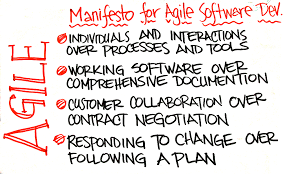
\includegraphics[width=.6\textwidth]{img/agile.png}
	\caption{Manifesto for Agile Software Dev.[www.medium.com]}.\label{rys:agile}
\end{figure}

Manifest przedstawia pewien system wartości, definiuje rzeczy najistotniejsze w zarządzaniu projektem.
Mamy więc cztery porównania:

\begin{itemize}
	\item Autorzy Manifestu stwierdzili, że ludzie i interakcje między nimi są ważniejsi,
	niż procesy i narzędzia. To nie znaczy, że procesy i narzędzia nie są istotne,
	ale są mniej ważne. Trzeba położyć większy nacisk na ludzi i na interakcje pomiędzy nimi.
	To powoduje bardziej nieformalną komunikację, jej przyspieszenie, co się przekłada
	na szybsze i bardziej elastyczne realizowanie zadań i umożliwia bardziej
	elastyczne realizowanie tych zadań, kiedy zmieniają się warunki.
	\item Druga zasadą jest orientacja bardziej na działające oprogramowanie niż na dokumentację.
	Jeśli zerkniemy do starych wersji oprogramowania z lat 80-tych, 90-tych,
	do każdego programu dodawana była gruba instrukcja.
	Dzisiaj już o tym zapomnieliśmy. Dzisiaj wiele aplikacji nie ma w ogóle nawet instrukcji,
	a więc mówimy, że działają intuicyjnie (przynajmniej powinny).
	Dzięki temu, że orientujemy się na realizację tych najważniejszych efektów w projekcie,
	możemy lepiej wykorzystać zasoby, możemy szybciej osiągnąć te efekty, a rzeczy mniej ważne,
	mniej istotne, takie jak szczegółowa dokumentacja (jakaś dokumentacja przecież musi być),
	możemy odłożyć, możemy przeznaczyć dla nich mniejsze zasoby.
	\item Również jeśli chodzi o współpracę z klientem, w metodykach zwinnych
	proponuje się zmianę podejścia. Zamiast negocjować szczegółowo umowy,
	budujemy współpracę z tym klientem dlatego, że nie jesteśmy w stanie z góry przewidzieć,
	jaki będzie, tak do końca, zakres naszego projektu, co w tym projekcie zrealizujemy,
	co będzie potrzebne za rok, kiedy nasz produkt będzie prawie gotowy.
	Czy te wymagania się nie zmienią wielokrotnie, biorąc pod uwagę szybkość zmiany technologii,
	potrzeb, oczekiwań klientów, szybkość zmian na rynku. Zatem klient powinien być blisko,
	powinien dostarczać bieżące informacje o swoich potrzebach, a w kontrakcie zawieramy tylko te informacje,
	które są najważniejsze.
	\item I w końcu reagowanie na zmiany zamiast szczegółowego planowania.
	Oczywiście planowanie występuje w metodykach zwinnych, ale jest ono ograniczone tylko do tego,
	żeby dało się zarządzać takim projektem. Natomiast przede wszystkim orientujemy się na
	reagowanie na zmiany: zmiany potrzeb klienta, zmiany na rynku. Na dostosowanie naszego projektu,
	w kolejnych iteracjach, do tego, czego klient oczekuje.
\end{itemize}

Czasem niektórzy mówią, może żartobliwie, ale nieraz całkiem serio, że jeżeli czegoś nie zaplanowali,
to stosowali właśnie Agile. Nic bardziej błędnego: w Agile każda iteracja jest planowana,
w każdym dniu planujemy swoją pracę, stosujemy inne metody, rzadko stosujemy harmonogram Gantta,
ale także planujemy te działania. Zatem taki polski Agile („polnische Agile”, jak niektórzy mówią),
to przykład niewłaściwego zarządzania przedsięwzięciami i raczej nie należy się tym chwalić.
Warto jednak zauważyć, że nie do każdego projektu możemy zastosować metodyki zwinne.
One się lepiej sprawdzają wtedy, kiedy mamy:
\begin{itemize}
	\item bardzo krótkie, napięte terminy;
	\item projekty mają charakter unikatowy;
	\item są skomplikowane.
\end{itemize}

Mamy do zrealizowania coś nowego, nieoczekiwanego i mało czasu.
Wtedy ta metodyka zwinna rzeczywiście jest bardziej uzasadniona niż metodyki klasyczne.
Stosowanie metodyk zwinnych, szczególnie żądanie tej interakcji między pracownikami,
ogranicza nam wielkość zespołu, a więc ogranicza nam wielkość projektu.
Generalnie metodyki zwinne stosujemy:
\begin{itemize}
	\item w małych i średnich projektach, rzadziej w projektach dużych;
	\item konieczne jest, aby w metodyce zwinnej dostępny był dla nas klient,
	klient musi się na bieżąco kontaktować z nami i mówić czego potrzebuje,
	jakie są jego oczekiwania, czy jest zadowolony z tego, co uzyskuje w poszczególnych iteracjach;
	\item tematyka projektu musi być taka, aby klient z każdej iteracji miał jakąś wartość,
	bowiem staramy się często wypuszczać oprogramowanie, często wprowadzać nowe jego wersje,
	ale to powoduje, że ta nowa wersja musi dostarczyć jakąś wartość dla klienta.
\end{itemize}

W przypadku oprogramowania jest to oczywiste. W przypadku, kiedy budujemy jakiś budynek,
być może Agile wtedy nie jest aż tak przydatny.
Trzeba się zastanowić, czy możemy zastosować całą metodykę Agile,
czy jak współcześnie w wielu projektach, zastosować ją tylko w odniesieniu
do wybranych modułów projektu, tam, gdzie rzeczywiście ma ona zastosowanie.

Więcej informacji na temat metodyk zwinnych można znaleźć w~\cite{Cohen_2006}.



% !TeX program = latexmk
% !TeX spellcheck = pl_PL
% !TeX root = example.tex

\chapter{Najczęściej wykorzystywane narzędzia w zarządzaniu projektami}

Zarządzanie projektami informatycznymi ściśle wiąże się z wykorzystaniem narzędzi informatycznych,
które wspomagają ten proces. Przy ich wyborze warto pamiętać, iż mają pomagać w pracy projektowej,
a nie przeszkadzać w jej realizacji, dlatego należy wybierać je mądrze.
Przykładem nieodpowiedniego doboru narzędzia może być sytuacja,
w której kierownik projektu nie dotrzymuje terminów swoich prac,
ze względu na zajmowanie się raportowaniem postępu prac lub aktualizacją harmonogramu.
~\cite{Kopczewski_2015}

\section{Narzędzia wspomagające podejście klasyczne}

\subsection{Microsoft Project}

Najbardziej popularnym narzędziem stosowanym w metodykach klasycznych jest Microsoft Project (\ref{rys:project}).
Pozwala on na rozpisanie całego harmonogramu działań, zaplanowanie budżetu czy stworzenie wykresu Gantta,
tak niezbędnego w pracy kierownika. Pozwala także na tworzenie raportów, prezentacji i wykresów z postępów prac.

\begin{figure}[H]
	\centering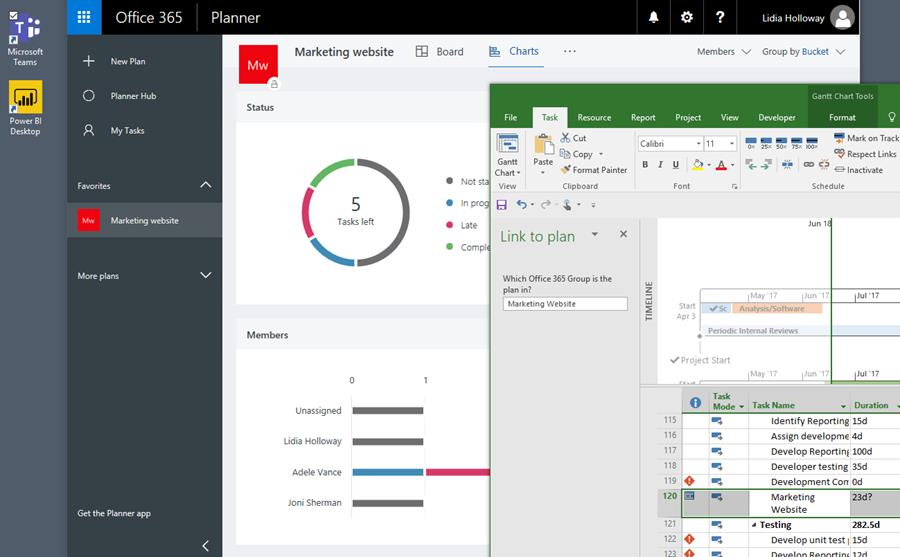
\includegraphics[width=.8\textwidth]{img/Microsoft_Project.jpg}
	\caption{Microsoft Project[www.microsoft.com]}\label{rys:project}% Źródło rysunku i etykieta przez którą odwołujemy się do rysunku.
\end{figure}

\subsection{Gantt Project}

W niektórych przedsiębiorstwach w zarządzaniu projektami używa się programu GanttProject.
Jest to darmowe narzędzie umożliwiające dynamiczne tworzenie diagramów Gantta
z podziałem na poszczególne zadania wraz z rozplanowaniem ich w czasie.
Dodatkowo pozwala ono na tworzenie wykresów PERT (ang. Program Evaluation and Review Technique)
wraz ze ścieżkami krytycznymi.
~\cite{Trendy_Zarzadzanie}

\section{Narzędzia stosowane w metodykach zwinnych}

W małych zespołach projektowych, które wykorzystują metodyki zwinne,
odchodzi się zazwyczaj od Microsoft Project czy GanttProject stosując aplikacje webowe.
Przykładem takich aplikacji są: Jira, Mantis, TFS, Trello, Redmine, Kanban Tool.

Przy metodykach zwinnych, właściciel produktu tworzy rejestr produktowy (ang. Product Backlog),
który ma formę listy zawierającej wymagania klienta z określoną wagą (priorytetem) i czasochłonnością.
~\cite{Shwaber_2004}

Wymienione wyżej narzędzia pozwalają na taką pracę i umieszczanie danych w chmurze,
dzięki czemu każdy członek zespołu ma do nich dostęp,
niezależnie od lokalizacji, czy pracuje w biurze czy poza nim.
Zadania w backlogu
\footnote{Backlog – rejestr sprintu / lista zadań~\cite{metody_zwinne_2016}}
powinny być rozpisane dla obecnego sprintu
\footnote{Sprint – jeden z etapów niektórych metodyk zwinnych, który wyznacza rytm pracy. W jego
trakcie następuje faktyczne wykonanie określonej funkcjonalności~\cite{Samoorganizacja_2010}}
oraz zawierać dodatkowe zadania, które będą zasilać kolejny sprint bądź zostaną wykonane w istniejącym,
gdy nadarzy się taka możliwość.

Takie podejście do pracy umożliwia wykonanie części zadań przed wyznaczonym czasem.
Narzędzia te pozwalają również na przypisanie konkretnego zadania do danego użytkownika,
dzięki czemu każdy pracownik zna zakres swojej odpowiedzialności.
Zapobiega to przypadkowemu wykonaniu tego samego zadania przez kilka osób.

Niektóre firmy, a można nawet powiedzieć, że wiele firm,
niezależnie od wykorzystywanej metodyki używa narzędzie Microsoft Excel do zarządzania projektami.
Umożliwia ono przedstawienie danych w postaci tabeli oraz różnych grafów.
Każda firma może zarządzać nim na swój własny sposób, dzięki czemu proces ten jest bardzo elastyczny.
Ponadto ułatwia on wykonanie prognoz przyszłych dochodów, kalkulacji wybranych parametrów i wskaźników.

Kolejnym narzędziem wykorzystywanym na szeroką skalę jest SharePoint,
który umożliwia współdzielenie plików czy tworzenie listy zadań,
która może być wykorzystana w MS Project.

\subsection{JIRA}

Jira to platforma do organizowania pracy i uruchamiania oraz monitoringu procesów w organizacjach.
Atlassian jest twórcą trzech produktów ściśle ze sobą powiązanych oraz wielu innych narzędzi również kompatybilnych z platformą Jira\cite{www_jira}

Rozwiązaniem dla zespołów wykorzystujących metodykę zwinną jest Jira Software.
Jest to narzędzie do zwinnego zarządzania projektami wsperające wszelkie metodyki zwinne w tym scrum,
kanban oraz metodyki niestandardowe.
Korzystając z takich funkcji jak tablice metod zwinnych czy raporty,
użytkownik może planować,
śledzić i zarządzać wszystkimi projektami zwinnego tworzenia oprogramowania w jednym narzędziu.~\cite{www_agile_jira}

Większość organizacji wykorzystuje platformę Jira do organizacji działów IT,
lecz coraz większa liczba przedsiębiorstw zaczyna rozszerzać systemy Jira
na obszary testowe i biznesowe m.in.\ takie jak marketing, dział prawny, HR lub finanse.
Dla wielu firm JIRA to jeden z najważniejszych systemów, które przechowują kluczowe informacje i
stanowią podstawę do podejmowania najważniejszych decyzji biznesowych.
Organizacje rozszerzają platformy JIRA za pomocą wyspecjalizowanych wtyczek (apps),
które są dostępne na Atlassian Marketplace oferującym ponad 2200 dodatków wykonujących różne funkcje.\cite{www_jira}

Jira jest więc zaawansowanym narzędziem do zarządzania projektami i nie tylko.
Pomaga ona też w zarządzaniu przedsiębiorstwami.
W dzisiejszych czasach gdzie przepływ informacji jest bardzo waćny jira stanowi bardzo pomocne narzędzie.

\begin{figure}[H]
	\centering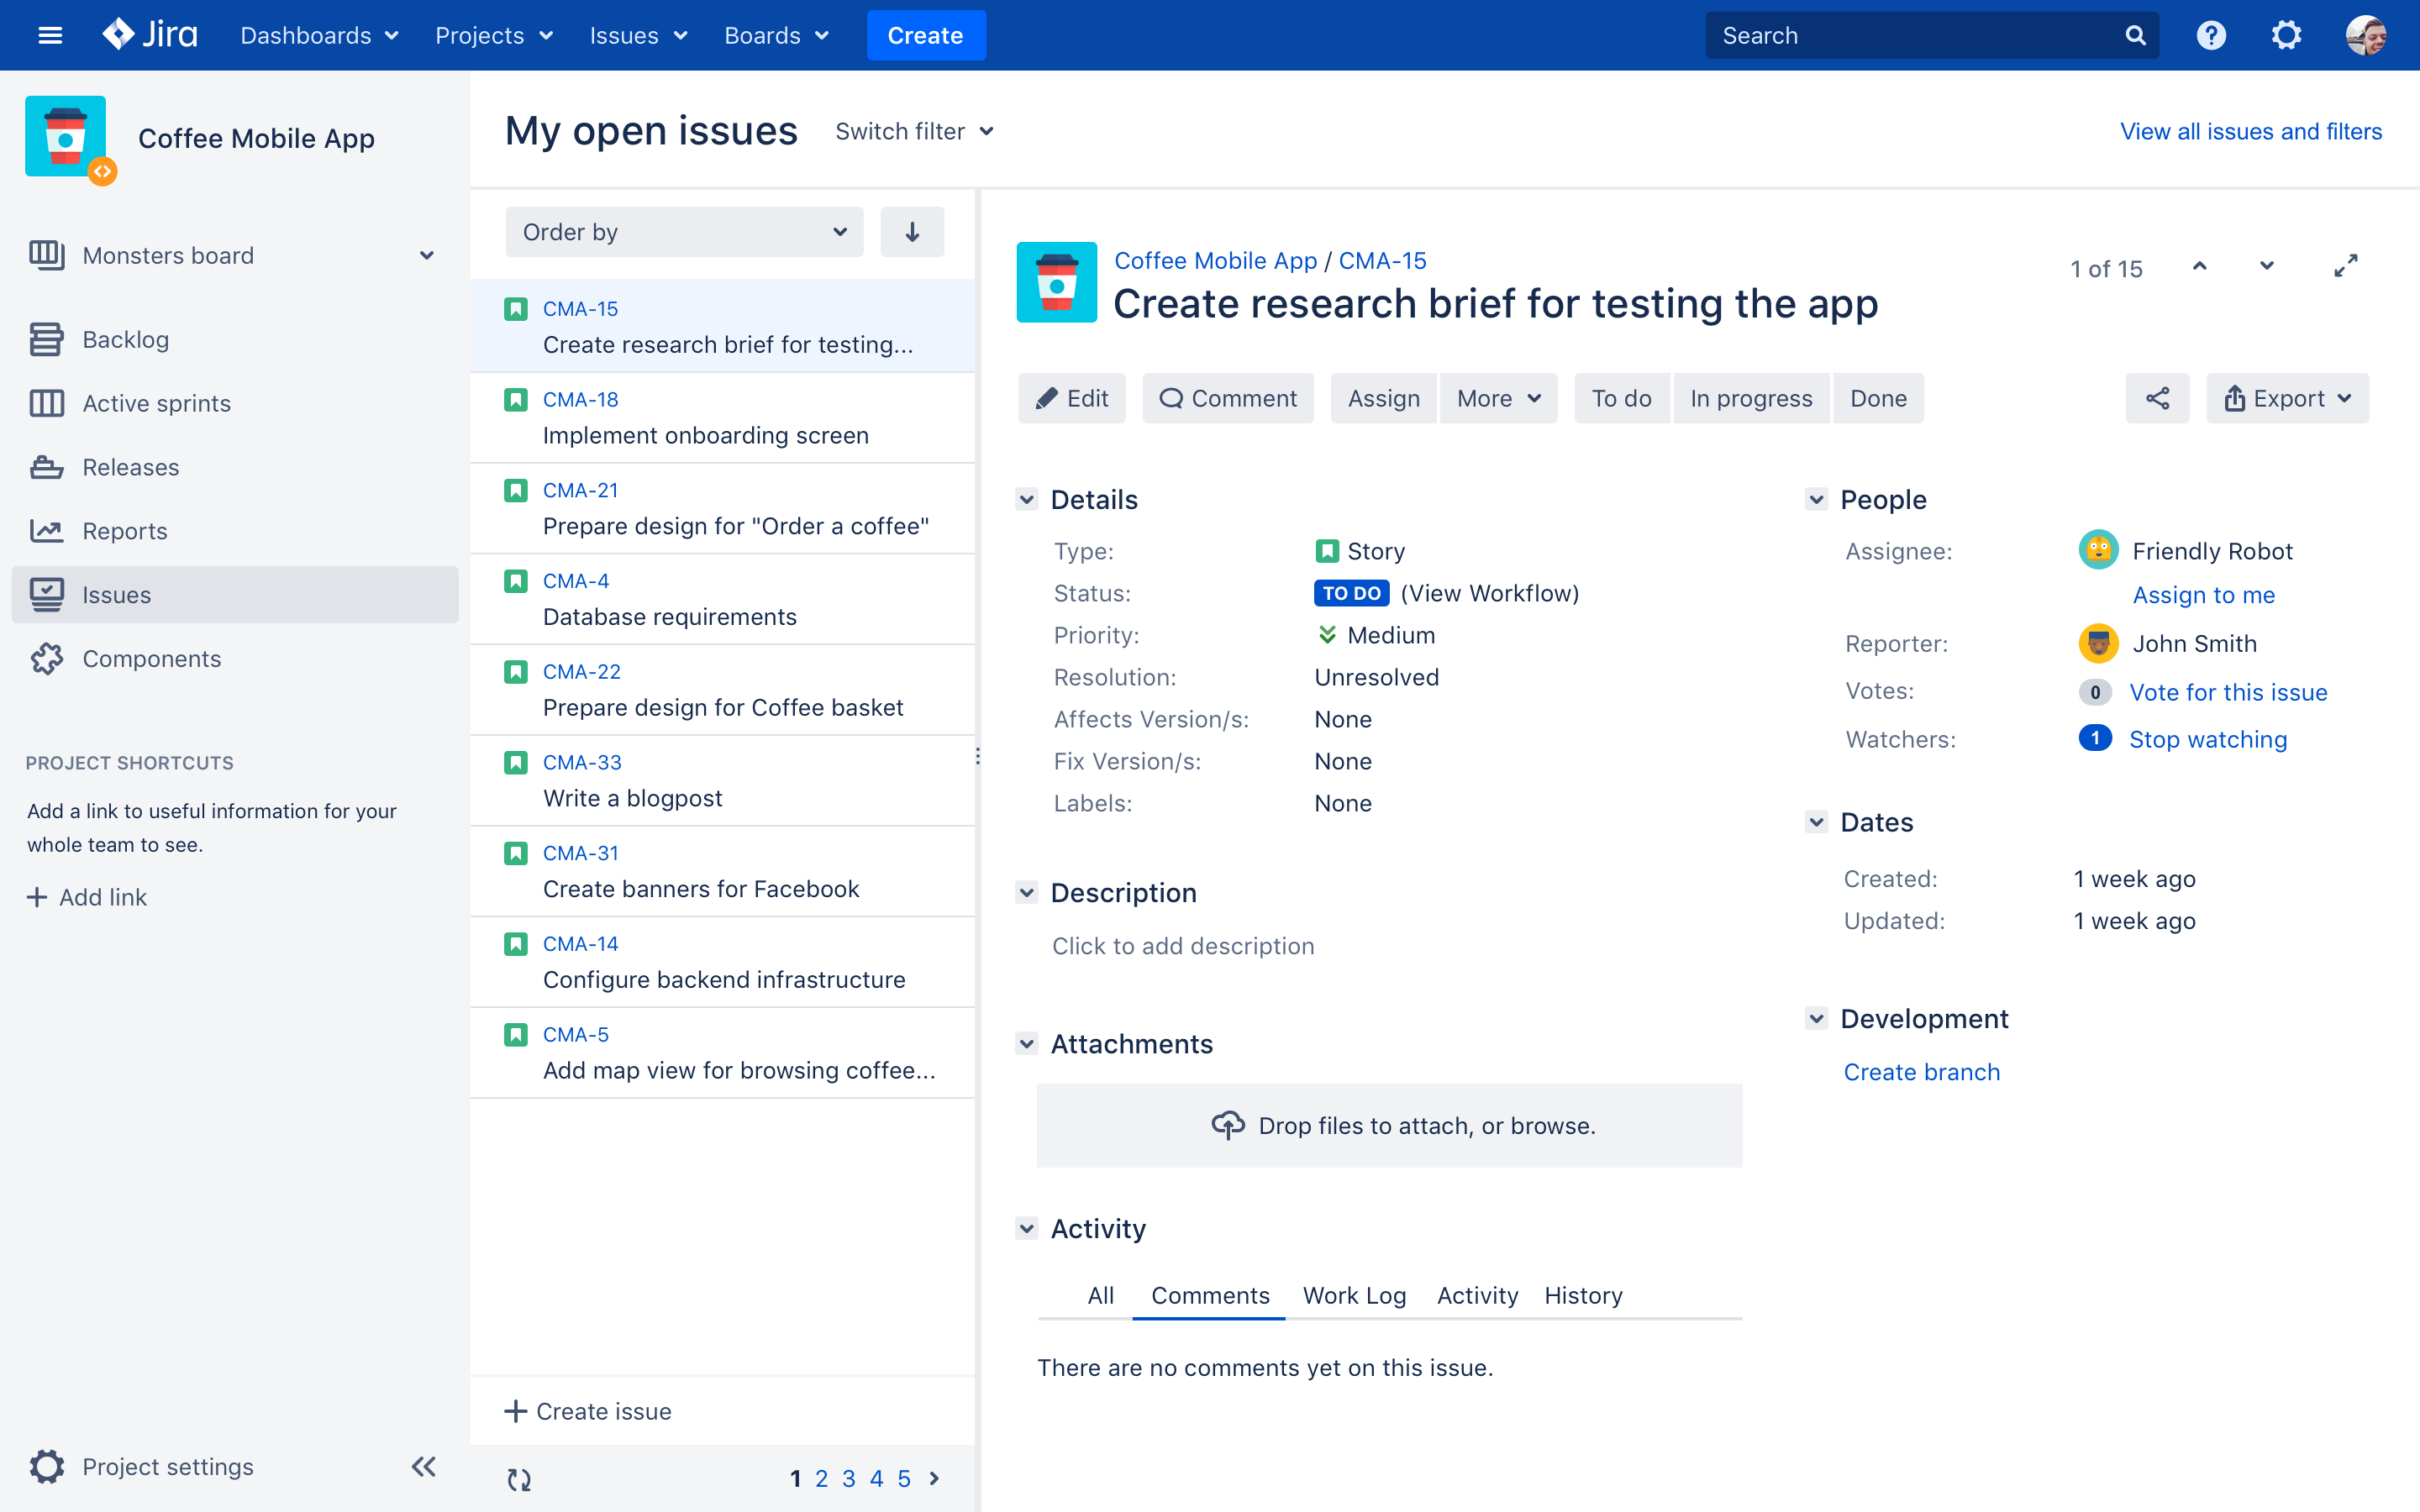
\includegraphics[width=.8\textwidth]{img/jira.png}
	\caption{Jira[www.jira.com]}\label{rys:trello}% Źródło rysunku i etykieta przez którą odwołujemy się do rysunku.
\end{figure}

\subsection{Trello}

Trello to na pierwszy rzut oka prosta aplikacja do zarządzania projektami,
która wszelkie dane przechowuje w postaci tablic.
Jednak karty, które w aplikacji pełnią rolę zadań posiadają wszelkie funkcję potrzebne do zarządzania.
Na przykład karty mogą przypominać o terminach, przechowywać listy zadań,
dzięki temu można śledzić progres zadania.

\begin{figure}[H]
	\centering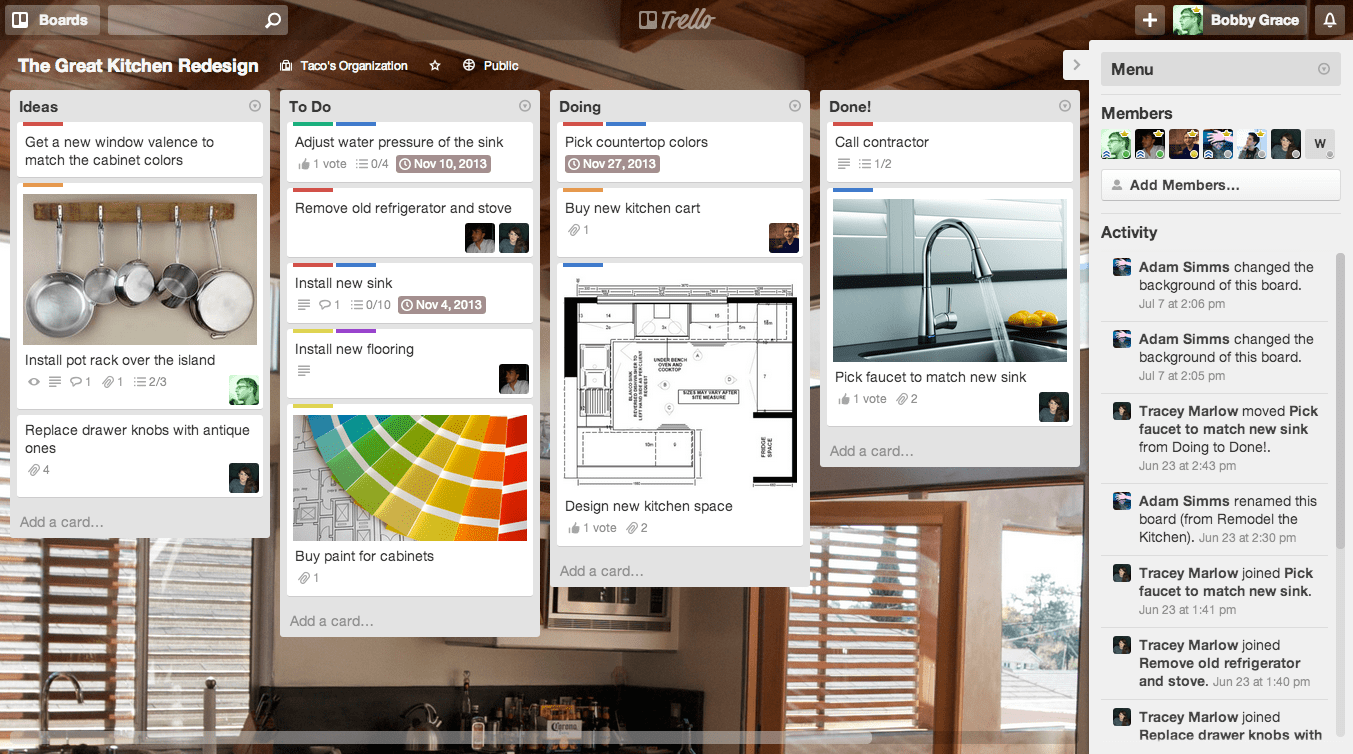
\includegraphics[width=.8\textwidth]{img/01.png}
	\caption{Trello[www.trello.com/home]}\label{rys:trello}% Źródło rysunku i etykieta przez którą odwołujemy się do rysunku.
\end{figure}

\section{Narzędzia wspomagające proces estymacji zadań projektowych}

W klasycznych projektach tworzymy harmonogramy, szczegółowe plany, gdzie mamy daty,
gdzie mamy godziny, gdzie każde zadanie ma określony czas realizacji.
W przypadku projektów zwinnych często odchodzimy od tak szczegółowego planowania.
ale jakaś forma planowania oczywiście jest potrzebna.
W projektach zwinnych bardzo często planujemy bez użycia dni i godzin.
Dlatego stosujemy różne alternatywne metody i jedną z takich alternatywnych metod
jest metoda zwana Team Estimation Game.

\subsection{Team Estimation Game}

Team Estimation Game w następujący:

\begin{itemize}
	\item Członkowie zespołu kolejno pobierają kartę ze stosu i przyklejają ją do ściany.
	Każda karta przedstawia jedną historyjkę.
	Po umieszczeniu pierwszej karty w środku, każdy członek zespołu umieszcza swoją kartę po prawej,
	jeśli jest trudniejsza, po lewej, jeśli jest mniej trudna,
	lub pod inną kartą, jeśli historyjki są mniej więcej takiej samej złożoności
	(patrz~\ref{rys:teamEstimationGame}).
	\item Użytkownik może użyć swojej kolejki, aby przesunąć kartę już na ścianie po prawej lub lewej stronie.
	\item Proces może być kontynuowany po tym, jak stos kart zostanie zużyty,
	aż do ogólnego konsensusu w rankingu kart. Gracze mogą omawiać historie i wpływać na swoje decyzje.
	\item Następnie każdy członek drużyny odbiera kartę z numerem i umieszcza ją na jednej z kolumn.
	Członek zespołu może użyć swojej kolejki, aby zmienić przypisanie numeru
	wykonane przez innego członka zespołu. Trwa to aż do osiągnięcia konsensusu.
\end{itemize}

\begin{figure}[H]
	\centering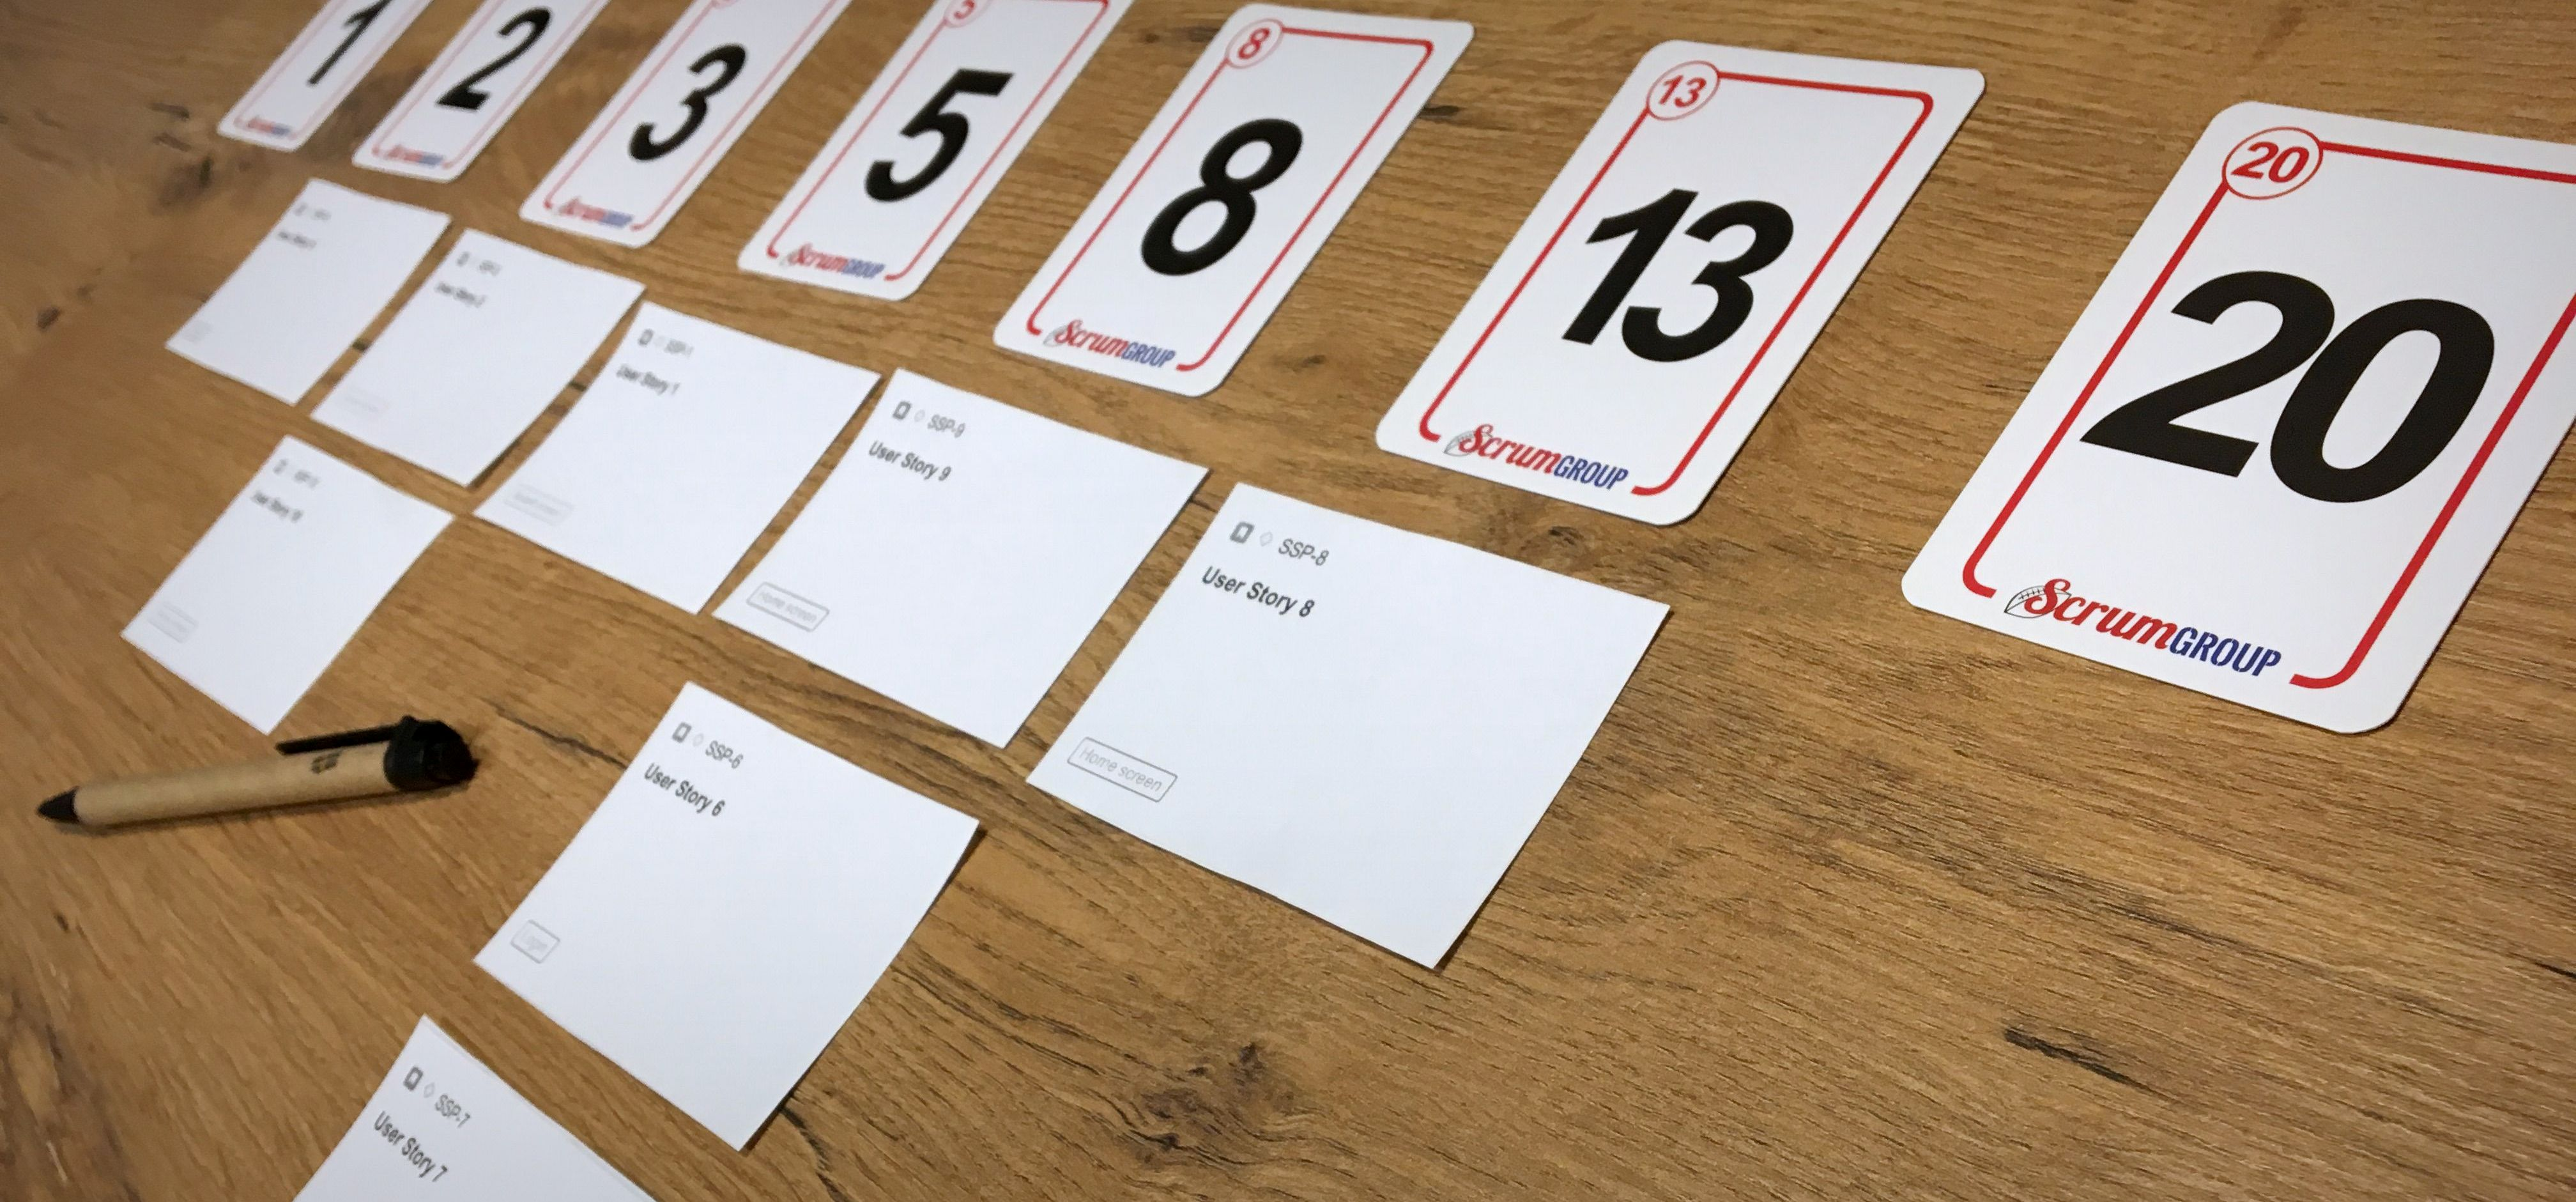
\includegraphics[width=.6\textwidth]{img/team_estimation_game.jpg}
	\caption{Team Estimation Game [www.scrum-master.pl]}\label{rys:teamEstimationGame}
\end{figure}

Zbiór liczb zawiera tylko te w sekwencji Fibonacciego, aby odzwierciedlić ogólną zasadę,
że ryzyko wzrasta geometrycznie proporcjonalnie do złożoności.

\subsection{Kanban}

Inną z takich alternatywnych metod jest metoda Kanban. Kanban, to koncepcja wzięta z produkcji,
która została świetnie zaadaptowana właśnie do zarządzania projektami zwinnymi.
Kanban w przypadku projektów jest po prostu tablicą, na której pokazujemy,
rejestrujemy to, co się dzieje w projekcie (patrz~\ref{tabela:kanban}).

Zaczynając od lewej strony tej tablicy, mamy backlog produktu, a więc wszystkie nasze historyjki,
które określają to, co jest w projekcie do realizacji.
Następnie mamy trzy główne etapy realizacji projektu, w których nasze historyjki będą się za chwilę znajdowały:

\begin{itemize}
	\item Pierwszym takim etapem jest \textit{breakdown} albo \textit{analysis}, czyli analizowanie historyjek,
	rozbijanie ich na mniejsze części, na zadania, analiza tego co jest do zrobienia, w jaki sposób mamy te zadania zrealizować.
	W tym miejscu musimy także zastanowić się nad kompatybilnością i powiązaniami pomiędzy poszczególnymi zadaniami,
	a także nad priorytetami. Dlatego bierzemy przede wszystkim te rzeczy, które mają wysoki priorytet oraz wszystkie funkcje,
	które są z nimi powiązane, abyśmy mogli dostarczyć nowy produkt.
	\item Kolejny etap, to jest rozwój (ang. \textit{develop}), który występuje w sytuacjach, gdzie opracowujemy nasz projekt,
	a więc tutaj zespół tworzy faktycznie te rozwiązania, które miały być opracowane.
	\item Trzeci etap, to \textit{validate}, czyli kontrola, testy, ocena tego, co zostało zrobione.
	Sprawdzamy czy rzeczywiście to, co miało być osiągnięte, zostało osiągnięte.
	Jeżeli tak, możemy dołączyć te funkcjonalności do produktu i przekazać je do klienta.
\end{itemize}

W każdym z tych etapów widzimy co najmniej dwie kolumny:

\begin{itemize}
	\item jedna kolumna, to \textit{working}, czyli pracujemy nad czymś,
	\item druga kolumna, to \textit{done}, czyli `wykonane' co oznacza wykonaliśmy to zadanie
	i dalej zadanie może przejść do kolejnego etapu, do kolejnej części prac.
	\item Dodatkowo, w przypadku kolumny związanej z rozwojem, mamy taką kolumnę \textit{track}
	– to sytuacja, w której opracowaliśmy jakąś funkcjonalność,
	ale nie jesteśmy jej w stanie wdrożyć dalej, ponieważ czekamy na opracowanie innych,
	powiązanych z nią funkcjonalności.
	Czasem jest tak, że pewna funkcjonalność może być już gotowa, ale nie może działać,
	dopóki inne elementy nie zostaną przygotowane.
	Dlatego jest takie pole oczekiwania na inne elementy, które muszą być przygotowane.
\end{itemize}

\begin{table}
	\centering\caption{Tablica w metodzie Kanban.}\label{tabela:kanban}
	\begin{tabular}{*8{l} }% wyrównanie kolumn tabeli -> l c r - do lewej, środka, do prawej
	\toprule
	\multicolumn{1}{|c|}{\textbf{Backlog}} &\multicolumn{2}{|c|}{\textbf{Breakdown (10*)}} & \multicolumn{3}{|c|}{\textbf{Develop (15*)}} & \multicolumn{2}{|c|}{\textbf{Validate (10*)}} \\
	\midrule
	Epics,User Stories & Working
	& Done & Working & Track & Done & Working & Done \\
	\bottomrule
	\end{tabular}
\end{table}

Widzimy więc, że w tej metodyce nie mamy iteracji jako takich, mamy stały przepływ historyjek,
stały przepływ pracy, która jest realizowana w naszym projekcie.
Ale ktoś może zapytać, w jaki sposób razie określamy poziom wykonania prac, w jaki sposób określamy
ile tej pracy możemy mieć jednocześnie rozpoczętej?
Temu służą te liczby w nawiasach, które widzimy w nagłówku tabeli.
Te liczby określają nam liczbę punktów, które mogą być aktualnie w obróbce.

Historyjki oceniamy nie względem czasu, lecz względem punktów trudności,
punktów zaangażowania, które jest niezbędne, aby daną funkcję zrealizować.
Jeżeli zatem w danym etapie naszej tablicy Kanban mamy dopuszczone 10 punktów,
to znaczy, że możemy tam mieć w trakcie obróbki historyjki,
których suma punktów estymacji nie przekracza 10-ciu. Tak samo w kolejnych etapach.
Zatem to określa nam poziom pracy, która jest wykonywana i powoduje, że praca będzie przebiegać płynnie,
nie będzie korków, nie będzie zatrzymań i będziemy w stanie w odpowiednim czasie dostarczać klientowi
nowe produkty.

\subsection{Planning Poker}

Jeszcze inną z takich alternatywnych metod (bardzo popularną) jest metoda,
której poświęcona jest niniejsza praca.
Ta metoda nazywa się \textit{Planning Poker} i pozwala nam oszacować trudność,
czasochłonność poszczególnych zadań, które są do wykonania w ramach projektu.
Ta metoda ma też tą zaletę, że integruje zespół i pozwala uwzględnić różne punkty widzenia,
a także przyczynia się do lepszego zrozumienia zadań, które są do wykonania.
O co w tej grze chodzi? Bazujemy tutaj z grubsza na liczbach z ciągu Fibonacciego (patrz~\ref{rysunek:poker}).

Określamy trudność poszczególnych zadań wykorzystując kolejne liczby z tego ciągu: 1, 2, 3, 5, 8,13, 21 itd.
Jeżeli jakieś zadanie oceniliśmy na 5, to znaczy, że jest ono trudniejsze od zadania, które oceniliśmy na 3,
ale ile ono zajmie? Tego nie wiemy, to nas chwilowo nie interesuje.
Staramy się określić, przede wszystkim, na ile trudne i na ile pracochłonne, naszym zdaniem, mogą być zadania.

Praktyka pokazuje, że planując sprinty, wcale nie musimy mieć szczegółowych informacji na temat czasu,
te informacje zresztą często się nie sprawdzają.
Taka forma punktowa zupełnie nam wystarcza. Kiedy wiemy, ile jesteśmy w stanie w ciągu sprintu
zrealizować takich punktów, to wówczas jesteśmy w stanie stwierdzić, ile możemy zadań w danym sprincie upchnąć.

Rozgrywka Planning Poker odbywa się następująco:

\begin{itemize}
	\item Zespół programistów spotyka się na spotkaniu, siada przy stole,
	każdy otrzymuje swoje karty i mamy pakiet zadań (czy pakiet historyjek) z backlogu,
	którymi się musimy zająć.
	Zazwyczaj spotkanie prowadzi scrum master lub właściciel produktu (ang. Product Owner),
	przedstawia on historyjkę, którą mamy się zająć, określa czego ona dotyczy.
	\item Następnie każdy z członków zespołu wyciąga kartę, która jego zdaniem dobrze określa trudność,
	realizacji tego zadania i kładzie ją na stole tak, aby nie było widać tej liczby.
	\item Kiedy wszyscy są gotowi, odwracamy karty i patrzymy czy wynik, który uzyskaliśmy jest zgodny,
	czy też nie. Jeżeli wszyscy pokazali praktycznie tą samą liczbę, to sprawa jest załatwiona.
	To znaczy, że wszyscy rozumiemy zadanie w taki sam sposób, tak samo oceniamy jego trudność
	i możemy przejść do kolejnego.
	\item Kiedy jednak występuje zróżnicowanie, konieczna jest dyskusja.
	Pytamy osoby, która podała najniższą liczbę, dlaczego tak uważa.
	Pytamy osoby, która podała najwyższą liczbę, dlaczego tak uważa.
	Bardzo często te różnice wynikają z tego, że nie do końca rozumiemy zadanie.
	Po dyskusji, gdy żaden z członków zespołu nie ma już wątpliwości co do
	szczegółów omawianego zadania, można powtórzyć rozgrywkę, która zazwyczaj dzięki
	odbytej dyskusji, kończy się konsensusem.
\end{itemize}

\begin{figure}[H]
	\centering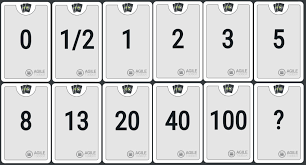
\includegraphics[width=\textwidth]{img/planningPokerCards.png}
	\caption{Przykładowe karty do Planning Pokera[www.scrumdesk.com]}\label{rysunek:poker}
\end{figure}

A więc Planning Poker pozwala nam lepiej zrozumieć zadania w zespole,
dzięki czemu nie ma później nieporozumień i dzięki czemu to planowanie jest bardziej precyzyjne.
Kiedy przejdziemy przez wszystkie historyjki i odzwierciedlimy, oszacujemy ich trudność w punktach,
możemy przejść do planowania sprintu.

Z doświadczenia wiemy, że nasz zespół jest w stanie zrealizować określoną liczbę punktów w ciągu danego sprintu.
Ta liczba nazywa się \textit{team velocity}, czyli szybkość, z jaką zespół pracuje.
Jest typowa dla każdego zespołu, a więc nie jest tak, że jeżeli jeden zespół
jest w stanie zrealizować 30 punktów, to każdy inny będzie w stanie tyle samo zrealizować.

Co więcej, nie można tej liczby traktować jako wskaźnika motywacji
(zróbcie pięć punktów więcej, to dostaniecie premię) dlatego,
że zaobserwowano, iż w takich przypadkach każde kolejne szacowanie po prostu powoduje,
że członkowie zespołu przydzielają więcej punktów, czyli określają zadania jako trudniejsze,
niż są w rzeczywistości, a więc mamy taką inflację punktów - nie ma realnego
zwiększenia realnego wykonanej pracy, jest po prostu zwiększenie liczby punktów.
Taki sposób motywacji nie jest zatem dobrym pomysłem.

Dzięki tej metodzie możemy odejść od określania, czy coś będzie trwało 2,5 godziny,
czy 3,5 godziny, możemy skupić się na lepszym zrozumieniu zadań,
jak również na tym, aby lepiej rozplanować pracę.


% !TeX program = latexmk
% !TeX spellcheck = pl_PL
% !TeX root = example.tex

\chapter{Rozproszone zespoły projektowe}

Według niemieckiego pisma \textit{Focus Money Magazin},
ok 30 \% wszystkich pracowników na świecie (a podobno w USA ponad 43 \%) pracuje w tzw.
zespołach rozproszonych lub wirtualnych.
Wiele firm wprowadza zarządzanie na odległość, aby w ten sposób stymulować rozwój,
rozwijać projekty międzynarodowe, czy chociażby ze względu na oszczędności lub optymalizację procesów.

Pojawienie się zjawiska zespołów rozproszonych może się wiązać z efektem globalizacji obszaru działania firm,
wkraczaniem na nowe rynki, powstawaniem \textit{startupów}, jak również działaniem tzw free-lancerów,
którzy oferują wyspecjalizowane usługi.
Powodem mogą być również wzrost kosztów pracy, zmiany na rynku pracy oraz brak na rynku lokalnym
wykwalifikowanych pracowników, jak również zmiany w kulturze pracy
(np.\ pokolenie tzw. Millenialsów). Wszystko to powoduje zmiany w organizacji pracy.

\section{Zalety zarządzania projektami w zespołach rozproszonych}

Realizacja projektów zespołami rozproszonymi:

\begin{itemize}
	\item pozwala na pozyskiwanie profesjonalistów w ramach całej organizacji lub poza nią;
	\item niweluje problem ograniczeń korzystania wyłącznie z zasobów jednego biura, czy w ramach jednego kraju;
	\item daje szerokie możliwości czerpania z dużo większych zbiorów doświadczeń oraz kreatywności;
	\item pozwala na elastyczność w rozbudowywaniu zespołu adekwatnie do pojawiających się nowych zadań;
	\item daje organizacjom szansę dostosowywania się do zmian pokoleniowych,
	gdzie często młode osoby wyrażają potrzebę wykonywania pracy w domu (ang. Home Office);
	\item zwiększa efektywność kosztową.
\end{itemize}

\section{Dodatkowe wyzwania dla efektywnego funkcjonowania zespołów rozproszonych}

Każdy zespół projektowy napotyka w swojej pracy na najróżniejsze wyzwania,
które związane są ze współpracą, komunikacją, czasami niejasnym podziałem obowiązków,
brakiem odpowiedzialności, czy zaangażowaniem.
Jednak zespoły rozproszone stają często przed dodatkowymi wyzwaniami, jakie wynikają z ich specyfiki,
czyli pracy w różnych lokalizacjach.

Oto kilka najczęstszych wyzwań takich zespołów:

\begin{itemize}
	\item \textbf{Zarzadzanie zespołem i synchronizacja pracy jego członków}

	To wyzwanie nie tylko dotyczy zespołów rozproszonych,
	ale w właśnie w takich zespołach szczególnie ważna jest umiejętność prowadzenia projektu
	i kwalifikacje związane z zarządzaniem ludźmi.
	W zespole rozproszonym powinny funkcjonować jasne zasady współpracy i komunikacji.
	Bardzo istotne jest ogólne zaangażowanie, wzajemne rozliczanie się z zadań,
	odpowiedzialność za rezultaty, otwartość, szacunek dla innych,
	zakładanie zawsze dobrych intencji, jasny podział obowiązków.
	Ważne jest również, dla budowania zespołu i jego efektywności, aby zaplanować
	(w budżecie oraz czasowo) okresowych, wspólnych spotkań wszystkich członków.

	\item \textbf{Przepływ informacji}

	Czasem kluczowe informacje nie docierają do wszystkich członków zespołu.
	Odpowiedzią na to może być ustalenie pewnego ``rytmu'' komunikacyjnego i regularne spotkania projektowe.
	Muszą to jednak być spotkania z sensem, tak zaplanowane, aby nie marnować czasu pracowników,
	aby rozwiązywały konkretne problemy i wspierały realizację celów projektu.
	Sposobów komunikacji jest wiele, można zatem je dobrze zaplanować i stosować,
	w zależności od złożoności zespołu, celu i rodzaju projektu.

	\item \textbf{Komunikacja w obcym języku}

	Coraz powszechniejsza jest konieczność porozumiewania się w języku obcym,
	ponieważ wiele firm posiada zagraniczne filie i siedziby.
	Zazwyczaj wykorzystywany do komunikacji jest język angielski,
	ale poziom jego znajomości może być różny i może powodować różne zabawne sytuacje lub nawet nieporozumienia.
	Tutaj może pomóc np.\ nauka prostych technik coachingowych czyli pytań doprecyzowujących i tzw.\ uważne słuchanie.
\end{itemize}

Dodatkowo zespoły rozproszone muszą się borykać z problemami takimi jak: różnica stref czasowych,
różnice kulturowe, odpowiednia rekrutacja, motywowanie i wsparcie zespołu, efektywność i produktywność,
zwiększa efektywność kosztową.

Dochodzimy wreszcie do kwestii, której bezpośrednio dotyczy temat niniejszej pracy inżynierskiej.
Jest to wyzwanie:

\begin{itemize}
	\item \textbf{Wsparcie techniczne i merytoryczne}

	W zespołach rozproszonych wręcz niezbędne jest zadbanie o wsparcie techniczne.
	Co więcej, wielu menedżerów zarządzających zespołami rozproszonymi,
	wskazuje na potrzebę wsparcia merytorycznego,
	szczególnie w zakresie moderowania tzw.\ metodyk zwinnych (SCRUM).
	Świetne połączenie internetowe,	sprzęt, sale i programy do tele- i wideokonferencji,
	to powinien być standard w organizacjach, które pracują w zespołach wirualnych.
\end{itemize}


Więcej informacji o zespołach rozproszonych można znaleźć w~\cite{www_rozproszony}.


\chapter{Założenia projektowe}

Tematem pracy jest stworzenie aplikacji wspomagającej szacowanie historyjek metodą Planning Poker.
Aplikacja pozwoli na przeprowadzenie gry, której backlog będzie pochodził z serwisu Github,
a wyniki gry będą zapisywane jako etykiety opisujące poszczególne zadania w Github.

Aplikacja będzie synchronizowana z Githubem,
czyli że jeżeli jakieś zadanie będzie z niego usunięte, usunięte zostanie również
z aplikacji.

Gra będzie posiadała także możliwości zamknięcia danego zadanie oraz jego edycji.

Inną planowaną funkcją jest możliwość tworzenia własnej skali estymacji.

Gracze będą dodawani do gry przez dzielenie się linkiem,
jednakże właściciel będzie mógł gracza wyrzucić z gry.

\section{Wymagania funkcjonalne}

\begin{itemize}
    \item Logowanie przez Github
    \item Logowanie jako gość (anonimowe)
    \item Pobieranie historyjek z Github
    \item Synchronizacja z Github
    \item Możliwość tworzenia list z issues Github
    \item Możliwość tworzenia gry
    \item Możliwość zapraszania graczy
    \item Możliwość głosowania przez graczy
    \item Możliwość tworzenia własnej skali estymacji
    \item Możliwość komentowania każdej historyjki podczas gry
    \item Możliwość automatycznego przeliczania wyników
    \item Możliwość wyrzucenia gracza z gry przez właściciela
    \item Możliwość eksportu wyników gry w postaci historyjek do Github
\end{itemize}

\section{Wymagania niefunkcjonalne}

\begin{itemize}
    \item Oprogramowanie musi być responsywne i proste.
    \item Aplikacja powinna się uruchamiać w przeglądarce internetowej.
    \item Aplikacja powinna działać w najnowszych wersjach przeglądarek.
    \item Aplikacja powinna działać w czasie rzeczywistym.
    \item Serwer powinien obsłużyć co najmniej 200 połączeń użytkowników.
    \item Zapewnienie bezpieczeństwa danych.
\end{itemize}

\section{Sposób komunikacji}

Aby aplikacja mogła komunikować się w czasie rzeczywistym niezbędne jest wykorzystanie
technologii Websockets, dzięki której możliwa będzie dwukierunkowa asynchroniczna komunikacja.

\section{Wykorzystanie technologie}

Aplikacja zostanie napisana w języku EcmaScript 6, kompilowanego do JavaScript
z wykorzystaniem SCSS, JSX i HTML5.

Wybrany zestaw technologii:
\begin{itemize}
    \item Node.js - środowisko uruchomieniowe do tworzenia aplikacji
    \item Yarn - Manadżer pakietów
    \item React -  biblioteka do tworzenia interfejsu użytkownika
    \item Redux - biblioteka wspomagająca zarządzanie stanem aplikacji
    \item Bootstrap - framework SCSS do budowania responsywnych stron internetowych
    \item Webpack - narzędzie do opakowywania, kompilowania i minimalizowania kodu
    \item Firebase - platforma służąca jako backend aplikacji
\end{itemize}


\chapter{Projekt aplikacji}

W niniejszym rozdziale autor umieścił projekt aplikacji oraz bazy danych.

\section{Diagram przypadków użycia}

\begin{figure}[H]
	\centering\includegraphics[width=.9\textwidth]{img/useCase}
	\caption{Diagram przypadków użycia}.
	\label{rys:useCase}
\end{figure}

\textbf{Product owner chce się zalogować}

\begin{enumerate}
    \item System prosi użytkownika o zalogowanie.
    \item Użytkownik naciska przycisk.
    \item Dostawca usługi logowania loguje użytkownika lub prosi o dane logowana.
    \item Product owner zostaje zalogowany do systemu.
    \item Product owner przegląda listę swoich projektów.
\end{enumerate}

\textbf{Product owner chce stworzyć listę}

\begin{enumerate}
    \item Product owner loguje się do systemu.
    \item Product owner wybiera projekt dla którego chce stworzyć listę.
    \item Product owner wybiera elementy do nowej listy z 'Issues' Github'a.
    \item Product owner naciska przycisk do tworzenia listy.
    \item Product owner nadaje listę nazwę i potwierdza wybór historyjek.
\end{enumerate}

\textbf{Product owner chce stworzyć gre}

\begin{enumerate}
    \item Product owner loguje się do systemu.
    \item Product owner wybiera projekt dla którego chce stworzyć grę.
    \item Jeżeli w projekcie jest stworzona jakakolwiek lista system prosi product ownera o wypełnienie formularza,
    w przeciwnym razie system odsyła użytkownika do listy issue's Github'a w celu stworzenia listy.
    \item Użytkownik potwierdza swoje ustawienia.
    \item System tworzy grę i przekierowuje użytkownika do listy gier projektu.
\end{enumerate}

\textbf{Product owner chce przeprowadzić grę}

\begin{enumerate}
    \item Product owner loguje się do systemu.
    \item Product owner tworzy grę.
    \item Product owner wchodzi do gry.
    \item Product owner rozsyła link do gry graczom.
    \item Gracze głosują nad historyjką.
    \item Product owner zmienia historyjki nadając tempo grze.
\end{enumerate}

\textbf{Product owner chce zmienić dane historyjki}

\begin{enumerate}
    \item Product owner loguje się do systemu.
    \item Product owner wybiera projekt.
    \item Product owner naciska przycisk edit przy issue.
    \item Product owner edytuje issue.
    \item Product onwer potwierdza zmiany.
\end{enumerate}

\textbf{Product owner chce zmienić ustawienia gry}

\begin{enumerate}
    \item Product owner loguje się do systemu.
    \item Product owner wybiera projekt.
    \item Product owner wybiera gre.
    \item Product owner wchodzi do gry.
    \item Product onwer naciska przycisk ustawiena.
    \item Product owner przechodzi do ekranu ustawień gry.
    \item Product owner zmienia ustawienia.
    \item Product owner zatwierdza ustawienia.
    \item System zapisuje ustawienia w bazie.
\end{enumerate}

\textbf{Product owner chce usunąć gracza z gry}

\begin{enumerate}
    \item Product owner loguje się do systemu.
    \item Product owner wybiera projekt.
    \item Product owner wybiera grę.
    \item Product owner wchodzi do gry.
    \item Product owner naciska przycisk "Gracze".
    \item System wyświetla product ownerowi listę graczy.
    \item Product owner naciska przycisk usunięcia przy nazwie gracza.
    \item System usuwa gracza oraz wszystkie jego oceny z gry ponownie obliczając punktację.
\end{enumerate}

\textbf{Product owner chce wyeksportować punktację}

\begin{enumerate}
    \item Product owner loguje się do systemu.
    \item Product owner wybiera projekt.
    \item Product owner wybiera grę.
    \item Product owner naciska przycisk eksport obok przycisku usuwania gry.
    \item System wyświetla product ownerowi listę historyjek wraz z ich punktacją.
    \item Product owner zatwierdza punktację.
    \item System przenosi punktację historyjek w postaci etykiet do Github'a.
\end{enumerate}

\textbf{Product owner chce usunąć gre}

\begin{enumerate}
    \item Product owner loguje się do systemu.
    \item Product owner wybiera projekt.
    \item Product owner wybiera grę.
    \item Product owner naciska przycisk usuń.
    \item System usuwa grę z bazy.
    \item Gra znika z listy gier.
\end{enumerate}

\section{Interfejs}

Aby ułatwić implementację systemu, autor zamodelował ekrany aplikacji w postaci
tzw. makiet (ang. mockups):

\begin{itemize}
    \item Ekranu logowania
    \item Ekrany listy projektów
    \item Ekrany projektu wraz z bocznym menu (ekran pprzedstawiający issues)
    \item Ekran formularza tworzenia gry
    \item Ekran listy gier
    \item Ekran gry
\end{itemize}

Prototyp interfejsu użytkownika został stworzony dzięki narzędziu Visual Paradigm.

\begin{figure}[H]
	\centering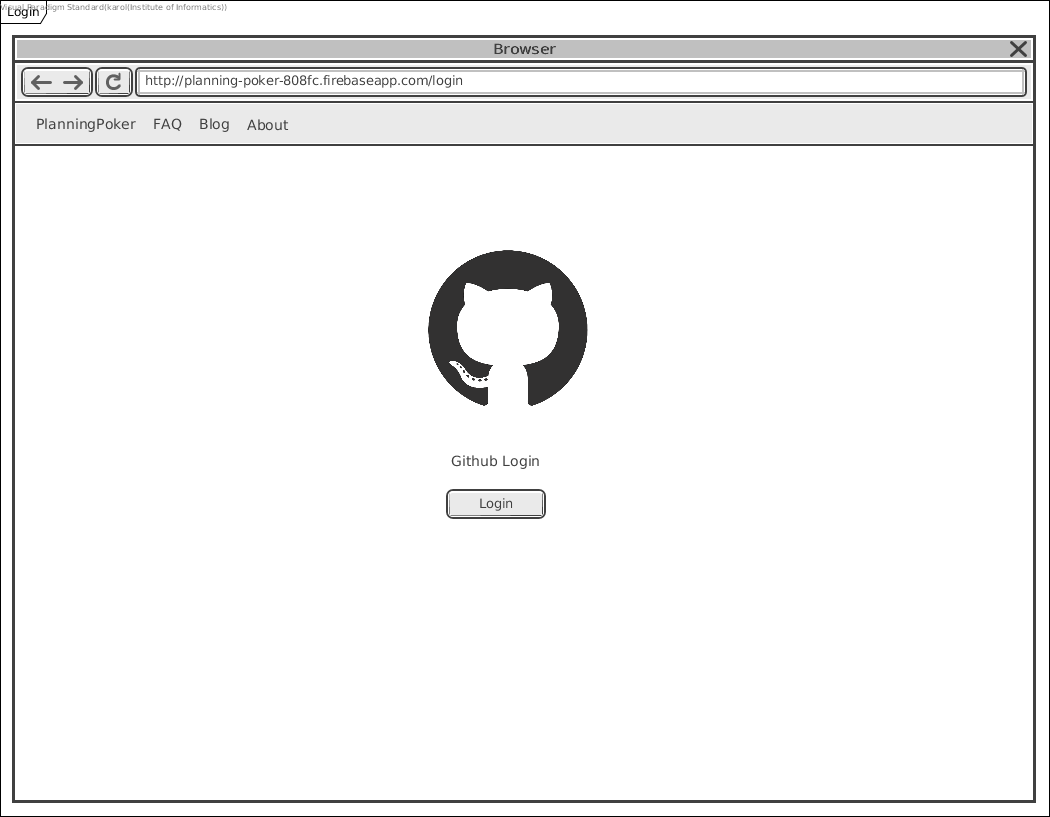
\includegraphics[width=.7\textwidth]{img/LoginScreen}
	\caption{Ekran Logowania}.
	\label{rys:loginScreen}
\end{figure}

\begin{figure}[H]
	\centering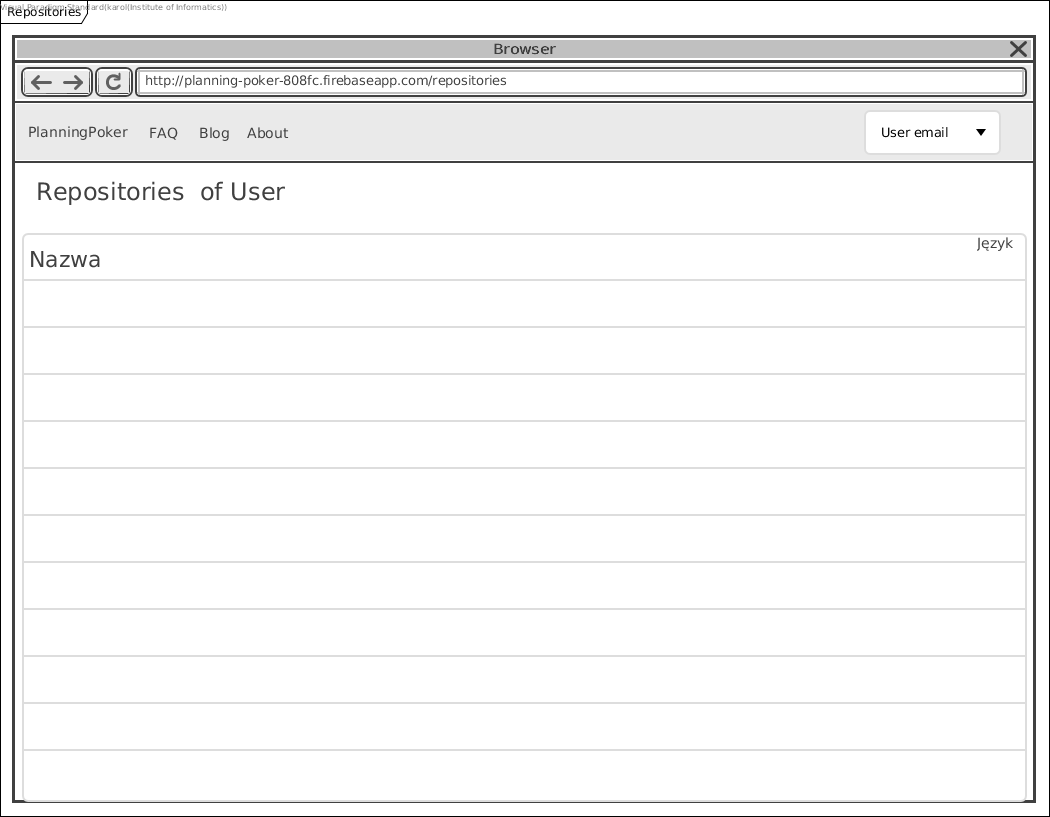
\includegraphics[width=.7\textwidth]{img/RepositoriesScreen}
	\caption{Ekran główny aplikacji z repozytoriami}.
	\label{rys:RepositoriesScreen}
\end{figure}

\begin{figure}[H]
	\centering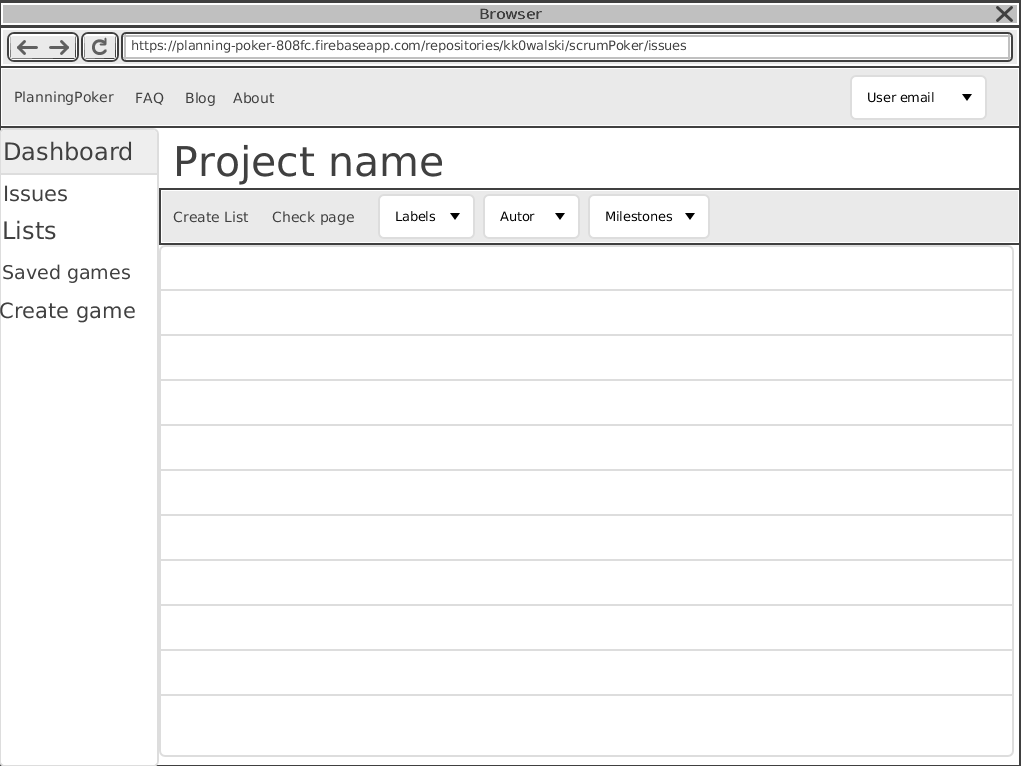
\includegraphics[width=.7\textwidth]{img/IssuesScreen}
	\caption{Główny ekran projektu}.
	\label{rys:IssuesScreen}
\end{figure}

\begin{figure}[H]
	\centering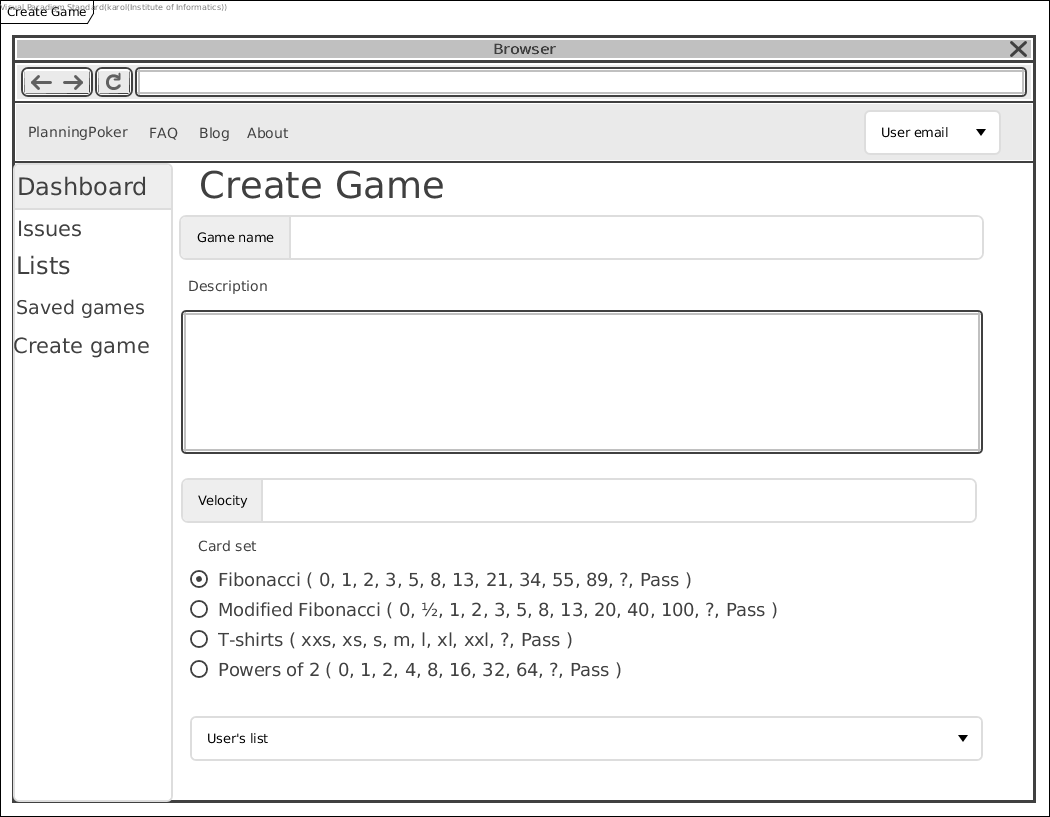
\includegraphics[width=.7\textwidth]{img/gameCreate}
	\caption{Formularz tworzenia gry}.
	\label{rys:gameCreate}
\end{figure}

\begin{figure}[H]
	\centering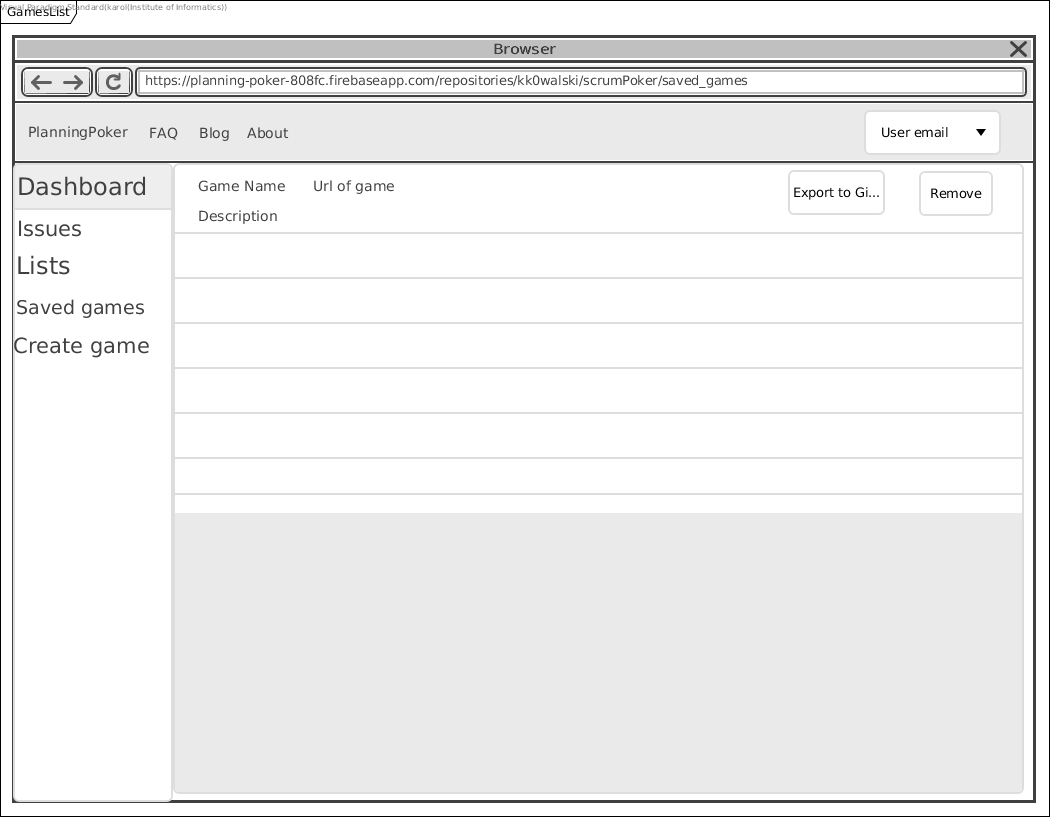
\includegraphics[width=.7\textwidth]{img/GamesList}
	\caption{Ekran gier}.
	\label{rys:GamesList}
\end{figure}

\begin{figure}[H]
	\centering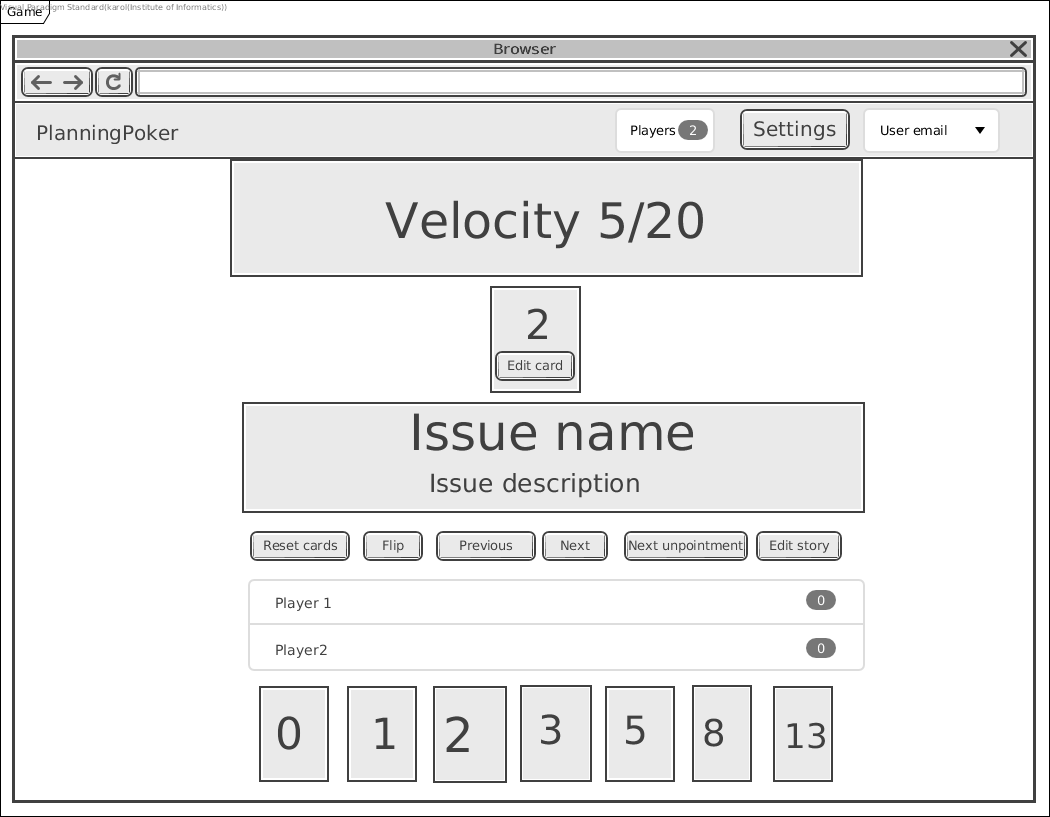
\includegraphics[width=.7\textwidth]{img/GameScreen}
	\caption{Panel gry}.
	\label{rys:GameScreen}
\end{figure}

Na rysunku \ref{rys:ScreensDiagram} przedstawiono diagram przepływu pomiędzy
zaprezentowanymi powyżej makietami ekranów aplikacji.

\begin{figure}[H]
	\centering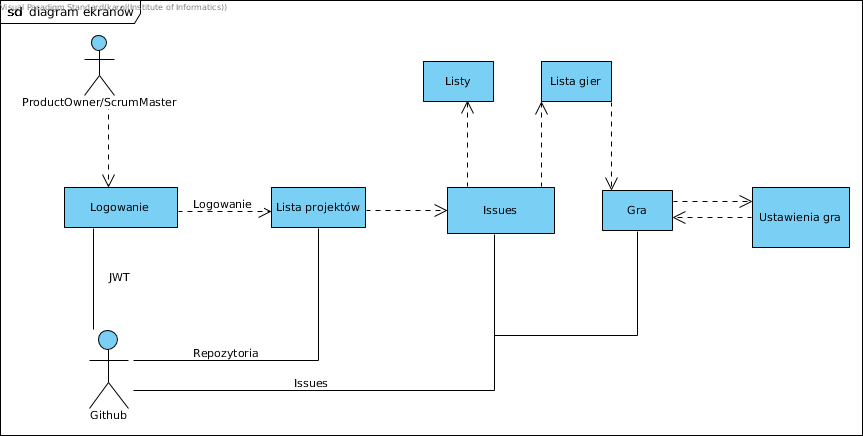
\includegraphics[width=\textwidth]{img/ScreensDiagram}
	\caption{Diagram przepływu między ekranami aplikacji}.
	\label{rys:ScreensDiagram}
\end{figure}

\section{Baza danych}

Na rysunku \ref{rys:ClassDiagram} przedstawiono model danych w aplikacji.

\begin{figure}[H]
	\centering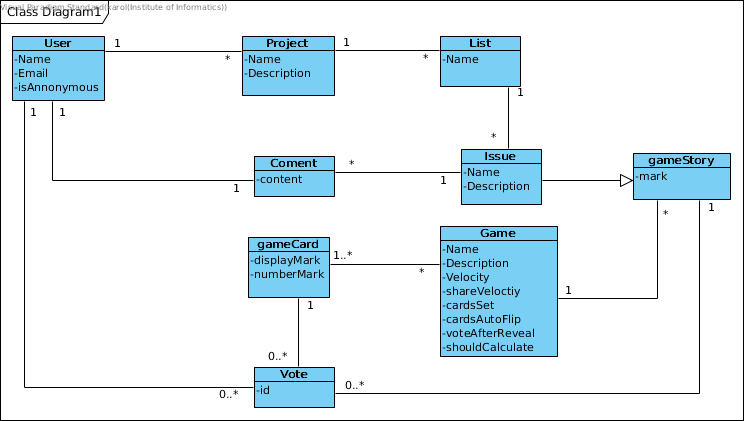
\includegraphics[width=\textwidth]{img/ClassDiagram}
	\caption{Diagram klas, przedstawiający koncepcję bazy danych}.
	\label{rys:ClassDiagram}
\end{figure}

W tym miejscu wartym odnotowania jest fakt, iż autor zdecydował się
na zastosowanie hierarchicznej bazy danych Firestore, zamiast którejś z najczęściej
wybieranych relacyjnych baz danych.

Ciekawym wnioskiem jest iż diagram klas UML z powodzeniem nadaje się do projektowania
modelu danych, który następnie może być zaimplementowany zarówno bazach
wykorzystujących relacyjny model danych (co autor miał już okazję robić
przy okazji innych projektów) jak również w przypadku bazy stosującej
model hierarchiczny.

Więciej o Firestore znajduje się w rozdziale o architekturze aplikacji.


% !TeX program = latexmk
% !TeX spellcheck = pl_PL
% !TeX root = example.tex

\chapter{Architektura aplikacji}

Projekt aplikacji wspomagającej zdalne szacowanie historyjek metodą Planning Poker
został wykonany w technologii, która pozwala na korzystanie z niej przy pomocy przeglądarki internetowej.

Architektura aplikacji oparta została o dwa podstawowe narzędzia:
ReactJS po stronie \textit{frontendu} oraz Firebase po stronie \textit{backendu}.
ReactJS to biblioteka napisana w języku JavaScript, stworzona przez firmę Facebook,
dzięki której budowanie dużych oraz kompleksowych interfejsów użytkownika staje się łatwiejsze.

Firebase z kolei to usługa świadczona przez firmę Google, która
pozwala na trwałe przechowywanie danych w chmurze, oferując przy tym
wsparcie dla obustronnej komunikacji protokołem Websocket, wykorzystywanym często
przez aplikacje internetowe wymagające interakcji pomiędzy użytkownikami w czasie rzeczywistym.

\section{Czym jest ReactJS}

Twórcy ReactJS opisują go jako Widok (ang. View) w architekturze MVC\@.
Wprowadza bardzo wydajny sposób utrzymania widoku zsynchronizowanego ze stanem danych
przechowywanym w pamięci przeglądarki w postaci obiektu Javascript.

Ten specjalny stos który renderuje HTML używa wyjątkowo szybkiego algorytmu opartego na wirtualnym drzewie DOM,
które jest ``lżejszym'' odpowiednikiem drzewa DOM\@. ReactJS wykorzystuje je
do minimalizacji liczby zmian w rzeczywistym drzewie DOM, potrzebnych do wprowadzenia go
w stan bezpośrednio wynikający z kształtu powiązanych danych.

Efektem tego algorytmu jest bardzo duża wydajność aplikacji korzystających z ReactJS oraz
łatwość pisania tych aplikacji ze względu na to, iż większością optymalizacji związanych
z renderowanie interfejsu użytkownika zajmuje się wspomniany algorytm.

Ponadto ReactJS ma jednokierunkowy, reaktywny przepływ danych,
który jest znacznie bardziej zrozumiały i łatwiejszy w rozwoju od podejścia tradycyjnego,
czyli wielokierunkowej komunikacji pomiędzy komponentami.

Komponenty – podstawowe bloki aplikacji React'owych – są zorganizowane w drzewie hierarchicznym,
w którym komponenty-rodzice wysyłają dane do swoich dzieci przez zmienne właściwości.
Każdy komponent ma także zmienną stanu, która determinuje obecne dane dla tego widoku.
Za każdym razem, gdy stan jest zmieniany, komponent wywołuje metodę \textit{render},
a React znajduje najbardziej efektywną metodę aktualizacji drzewa DOM\@.

Odkąd głównym zadaniem React’a jest interfejs użytkownika,
aplikacje na nim zrobione potrzebują czegoś jeszcze,
co będzie zachowywało się jak tzw. \textit{backend}, czyli sposób na trwałe
przetrzymywanie danych, nieleżne od stanu przeglądarki, która służy jako
środowisko uruchomieniowe dla ReactJS\@.
Do tego celu zdecydowałem się na użycie usługi Firebase.
Firebase dostarcza model (ang. Model) i kontroler (ang. Controller) w MVC
do aplikacji napisanych w ReactJS, czyniąc z nich w pełni funkcjonalne aplikacje,
których stan nie zależy wyłącznie od przeglądarki internetowej, w której działają.
Używając React’owego jednokierunkowego systemu wiązania danych łatwo jest zintegrować go z Firebase.
~\cite{www_react}

\section{Firebase}

Firebase jest platformą dla aplikacji webowych oraz mobilnych, która wprowadza
dla deweloperów mnóstwo narzędzi oraz usług pomagających im tworzyć wysokiej jakości
aplikacje oraz zwiększyć ich bazę użytkowników.

\subsection{Historia Firebase}

W 2011 roku Firebase znany był pod nazwą Envelope.
Jako Envelope wprowadził dla deweloperów API,
które umożliwiało wprowadzenie komunikatora do ich strony internetowej.

Interesującym było to, że ludzie używali aplikacji by przekazywać dane,
które były czymś więcej niż wiadomościami komunikatora.
Deweloperzy aplikacji internetowych (w tym gier) używali Envelope
w celu synchronizacji danych aplikacji jak i stanu gry
w czasie rzeczywistym pomiędzy ich użytkownikami.

To doprowadziło założycieli Envelope, Jamesa Tamplina oraz Andrew Lee
do pomysłu by rozdzielić komunikator online oraz platformę wymiany danych w czasie rzeczywistym.
W kwietniu 2012 Firebase powstał jako oddzielna firma które wprowadziła usługę backendu
(ang. BaaS, Backend-as-a-Service) z funkcjonalnościami czasu rzeczywistego.

Po tym jak firma została przejęta przez Google w 2014 roku,
szybko ewoluowała do wielofunkcyjnej platformy mobilnej oraz webowej jaką znamy dzisiaj.

\section{Usługi Firebase wykorzystane w pracy}

% Rysunek
\begin{figure}
	\centering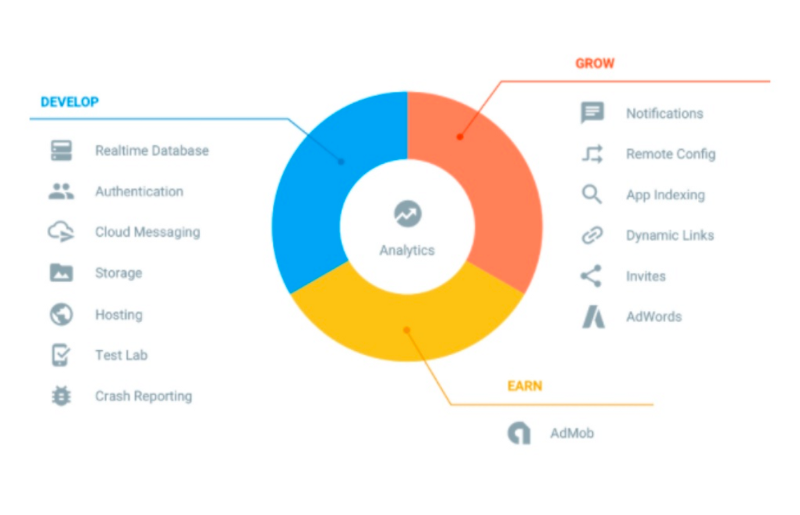
\includegraphics[width=.6\textwidth]{img/firebase}
	\caption{Usługi Firebase.[hackernoon.com]}\label{rys:firebase}% Źródło rysunku i etykieta przez którą odwołujemy się do rysunku.
\end{figure}

\subsection{Firebase Authentication}

W swojej aplikacji przede wszystkim skorzystałem z usługi \textit{FireBase Authentication},
która wprowadza usługi serwerowe,
łatwe narzędzia dla deweloperów oraz biblioteki Javascript
znacząco przyspieszające implementację oraz bezpieczeństwo
funkcji związanych z rejestracją oraz uwierzytelnieniem w aplikacji.

Autor skorzystał z usług logowania anonimowego oraz
tzw. \textit{third-party authentication} w usłudze Github, poprzez protokół OAuth.
Uwierzytelnienie poprzez usługę Github pozwala na integrację aplikacji z
narzędziem Github, co jest funkcją kluczową dla realizacji celu projektu.

\subsection{Firestore}

Firestore jest nierelacyjną bazą dokumentów, która pozwala łatwo przechowywać,
synchronizować oraz przeszukiwać dane w aplikacjach mobilnych oraz webowych – w globalnej skali.

Firestore przechowuje dane w postaci obiektów zwanych dokumentami.
Te dokumenty posiadają pary klucz-wartosć oraz mogą zawierać jakiekolwiek rodzaje danych
od łańcuchów po dane binarne a nawet obiekty, które przypominają format JSON\@.
Dokumenty są pogrupowane w kolekcje.
~\ref{rys:firestoreData}

\begin{figure}
	\centering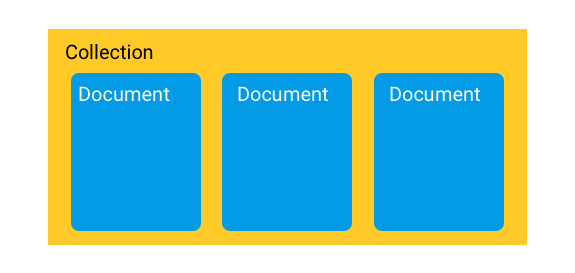
\includegraphics[width=.6\textwidth]{img/firestoreData}
	\caption{Postać danych w firestore [hackernoon.com]}\label{rys:firestoreData}% Źródło rysunku i etykieta przez którą odwołujemy się do rysunku.
\end{figure}

Fierstore może zawierać wiele kolekcji zawierających dokumenty, które wskazują na subkolekcje.
Te subkolekcje mogą znowu zawierać dokumenty oraz swoje subkolekcje i tak dalej.
Można zatem powiedzieć że jest to hierarchiczny model danych (patrz~\ref{rys:firestoreTree}).
~\cite{www_hakermoon}

\begin{figure}
	\centering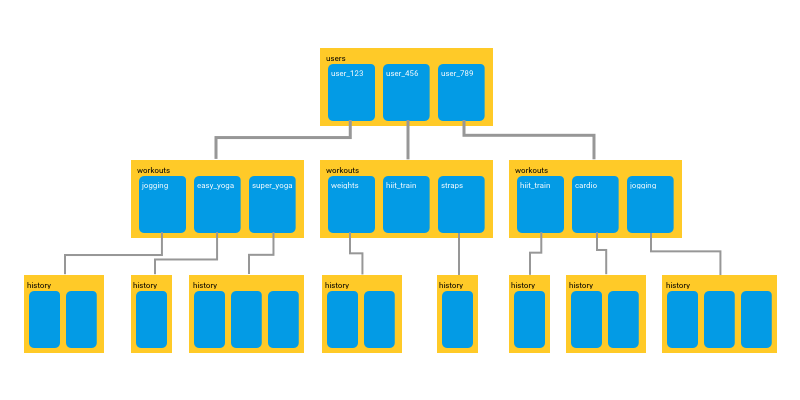
\includegraphics[width=.6\textwidth]{img/firestoreTree}
	\caption{Ułożenie danych w firestore [hackernoon.com]}\label{rys:firestoreTree}% Źródło rysunku i etykieta przez którą odwołujemy się do rysunku.
\end{figure}

\section{Redux czyli implementacja architektury Flux}

Jedną z najważniejszych cech komponentów ReactJS jest wbudowany w nie stan.
Jest to bardzo przydatna koncepcja. Komponent posiada stan,
który może ulec zmianie w wyniku interakcji użytkownika z aplikacją.
Zmiana stanu pociąga za sobą operację re-renderowania drzewa Virtual DOM\@.
W wyniku tego, pewne części interfejsu widocznego na ekranie ulegają zmianie.
Oczywiście wiadomym jest też, że jeden komponent może zależeć od innego komponentu.
Możemy przecież przekazywać stan komponentu rodzica do jego komponentów dzieci itd.

To wszystko działa świetnie. Niestety w miarę jak aplikacja rośnie,
rozrasta się poziom skomplikowania poszczególnych komponentów.
Z tego względu programiści Facebooka, odpowiedzialni za rozwój ReactJS, wymyślili
architekturę aplikacji, która rozwiązuje ten problem.
Architektura ta nazwa się \textbf{Flux}.
~\cite{www_nafrontendzie}

\subsection{Architektura FLUX}

Flux jest architekturą, której Facebook używa do budowania aplikacji po stronie klienta.
Jest to uzupełnienie komponentów React’a przez wykorzystanie jednokierunkowego przepływu danych.
Nie jest to gotowe narzędzie, czy biblioteka, lecz pewien wzorzec architektoniczny.
Można z niego korzystać bez wielu nowych linijek kodu.

\begin{figure}
	\centering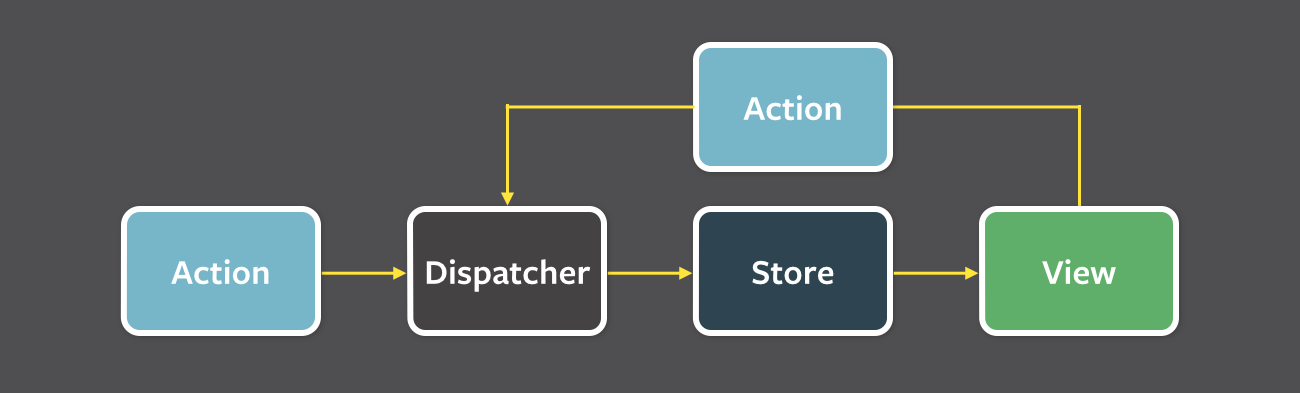
\includegraphics[width=.6\textwidth]{img/flux}
	\caption{Architektura Flux [wwww.nafrontendzie.pl]}\label{rys:flux}% Źródło rysunku i etykieta przez którą odwołujemy się do rysunku.
\end{figure}

Przepływ rozpoczyna się od lewej strony.
Najpierw tworzone jest akcja – jest to zwykły obiekt zawierający właściwość \texttt{type}.
Oprócz tego może on posiadać więcej właściwości służących do przekazywania dodatkowych danych.
Akcja taka tworzona jest przez funkcję zwaną \textit{action creator}, czyli kreator akcji.
W przypadku Redux, akcja jest zwykłą funkcją.

% lub {java} albo {bash} albo {text}
\begin{listing}
\begin{minted}{c}
const mapStateToProps = (state) => {
    return { counter: state.counter };
};
const mapDispatchToProps = (dispatch) => {
    return {
        onIncrement: () => dispatch({ type: 'INCREMENT' }),
        onDecrement: () => dispatch({ type: 'DECREMENT' })
    }
};

Counter = connect(mapStateToProps, mapDispatchToProps)(Counter);
\end{minted}
\caption{Przykładowe akcje licznika i ich stan} \label{listing:licznik}
\end{listing}

W listingu~\ref{listing:licznik} przedstawiony jest prosty licznik z dwoma akcjami,
które zwiększają bądź zmniejszają licznik o jeden.
Stan oraz funkcje rozsyłające dostępne są w obiekcie \texttt{this.props}.
Spójrzmy na kod odpowiedzialny za ich mapowanie.
\begin{center}
	\textbf{Funkcja mapStateToProps}
\end{center}
Funkcja \texttt{mapStateToProps} pobiera \texttt{state} jako parametr i zwraca nowy obiekt.
Częstą praktyką jest po prostu przekazanie całego stanu do właściwości,
jednak jest to też właściwe miejsce by odfiltrować dane.
\begin{center}
	\textbf{Funkcja mapDispatchToProps}
\end{center}
Kolejna funkcja to \texttt{mapDispatchToProps}. Zwraca ona obiekt zawierający metody.
Za pomocą wywołania funkcji \texttt{dispatch} rozgłasza ona obiekty akcji do \texttt{store}.
Metoda \texttt{dispatch} przekazuje obiekty akcji bezpośrednio.

Zwykle w projekcie definiuje się to jako specjalne kreatory akcji.
Dzięki kreatorom możemy opóźnić wywołanie akcji lub zmienić dane w naszym Redux tylko wtedy,
gdy są spełnione określone warunki (patrz~\ref{listing:firebase_action}).

% lub {java} albo {bash} albo {text}
\begin{listing}
\begin{minted}{c}
export const startAddUserToGame = (owner, repo, game, user = {}) => {
    return dispatch => {
        var userUpdate = {}

        const tempUser = {
            email: user.email,
            isAnonymous: user.isAnonymous,
            id: user.uid,
            name: user.displayName,
            online: true
        };

        userUpdate[`users.` + user.uid.toString()] = tempUser
        const gameRef = db
        .collection(`users`)
        .doc(owner.toString())
        .collection(`repos`)
        .doc(repo.toString())
        .collection(`games`)
        .doc(game.toString())

        gameRef.update(userUpdate).then(() => {
            dispatch(addUserToGame(owner, repo, game, tempUser))
        });
    }
}
\end{minted}
\caption{Przykładowy kreator akcji z projektu} \label{listing:firebase_action}
\end{listing}

W tym przykładzie gracz jest dodawany do gry tylko wtedy,
gdy jest uczestnikiem gry w bazie danych Firestore.
Jak widać w przykładzie, kreator zwraca funkcję,
która wykorzystuje \texttt{dispatch} by wysłać akcję do store.
Aby zadziałać, funkcja musi znać dokładną lokalizację gry w bazie oraz dane użytkownika.
Aby dostać się do gry, musimy znać właściciela oraz nazwę repozytorium w której znajduje się gra
oraz identyfikator gry.

Dzięki funkcji \texttt{update} gracz jest dodawany do gry dostając się odpowiednio do obiektu \texttt{users},
dokumentu gry, kolekcji repozytoria, dokumentu naszego repozytorium.
Kolekcja gier znajduje się w repozytorium, a dzięki znajomości identyfikatora gry
dostajemy się do jej obiektu i wstawiamy do niej obiekt gracza.
Jeżeli akcja w bazie danych zakończy się sukcesem, rozsyłamy akcję dodawania gracza do store.

\begin{center}
	\textbf{Funkcja connect}
\end{center}
Wracając do mapowania. W przedstawionym wcześniej przykładzie najbardziej istotna jest ostatnia jego linia.
Wywołuję ona funkcję \texttt{connect}.
Przyjmuje ona funkcje \texttt{mapStateToProps} oraz \texttt{mapDispatchToProps}
jako parametry i wyniki ich wywołania łączy w odpowiedni obiekt.
Następnie zwraca funkcję, która jako parametr przyjmuje komponent.
Funkcja ta wprowadza przygotowany wcześniej obiekt do \texttt{this.props} tego komponentu.

Funkcja connect opakowuje przekazany komponent i zwraca nową jego wersję.

Wracając do Flux. Tak tworzona akcja jest dostarczana do store za pomocą wywołania funkcji \texttt{dispatcher}.
Funkcja ta w zasadzie zarządza całym przepływem danych.
Każdy store w aplikacji rejestruje w dispatcherze swoje funkcje wywołania zwrotnego
w celu obsługi przychodzących akcji.
W momencie gdy akcja jest rozsyłana (ang.\ dispatch), wywoływane są po kolei wszystkie
funkcje wywołania zwrotnego (ang.\ callback).
Jeden z nich powinien umieć rozpoznać akcję po jej typie i być przygotowany na jej odpowiednią obsługę.

\begin{center}
	\textbf{Funkcja reducer}
\end{center}

W przypadku Redux'a rolę store'a pełni funkcja \textit{reducer}. Dzięki temu, że jest to funkcja,
można ją jednocześnie użyć jako funkcję wywołania zwrotnego,
którą store uruchomi w momencie gdy zostanie rozgłoszona jakaś akcja.
Funkcja ta przyjmuje dwa parametry: \texttt{state} oraz \texttt{action}.

Działa to tak: ktoś wywołuje akcję, obiekt \textbf{store} wywołuje funkcję \textbf{reducer},
przekazując do niej aktualny stan oraz akcję, \textbf{reducer}
sprawdza typ przekazanej do niej akcji i w zależności od tego jaki jest ten typ,
zwraca nową wersję obiektu stanu (patrz przykład~\ref{listing:reducer}).

\begin{listing}
\begin{minted}{c}
const reducer = (state, action) => {
    switch (action.type) {
        case 'INCREMENT':
            return { ...state, counter: state.counter + 1 };
        case 'DECREMENT':
            return { ...state, counter: state.counter - 1 };
        default:
            return state;
    }
};
\end{minted}
\caption{Przykładowy reducer licznika} \label{listing:reducer}
\end{listing}

W przykładzie, jeśli typ akcji to `INCREMENT' to zwracany jest nowy obiekt stanu,
który ma zwiększoną o jeden wartość atrybutu \texttt{counter}.
Jeśli natomiast typ akcji to `DECREMENT' to zwracany jest nowy stan z atrybutem
\texttt{counter} zmniejszonym o jeden.
Jeśli typ akcji jest w tym miejscu nieznany, wykonujemy domyślną (ang.\ default) operację, którą jest
przekazanie obiekt stanu w niezmienionej postaci.

Generalnie wszystkie obiekty store zawierają łącznie cały stan aplikacji.
Store zawiera implementację funkcji wywoływania zwrotnego,
która jest rejestrowana w ``dispatcherze'', i która obsługuje akcje związane z danym store.
Cechą Reduxa jest to, że cały stan jest przechowywany w jednym obiekcie.

Kolejny element na diagramie to widok.
Można powiedzieć, że jest on reprezentowany po prostu przez komponent ReactJS\@.
Używa on stanu aplikacji zapisanego w obiekcie store, tak jakby był on wewnętrznym stanem komponentu.
Zmiana stanu w store powoduje re-renderownie komponentu.
Dodatkowo komponent widoku może rozsyłać kolejne akcje, na przykład kiedy użytkownik
kliknie na jakiś przycisk interfejsu na ekranie.
To powoduje zmianę stanu zapisanego w store.
W Redux komponent ma dostęp do akcji i stanu dzięki wspomnianej przeze mnie wcześniej funckji \texttt{connect}.

Wszystko to po prostu zestaw zasad.
To programista może zdecydować jak to dokładnie będzie zaimplementowane.
Na szczęście nie jest on zdany sam na siebie, ponieważ istnieje kilka gotowych
implementacji architektury Flux w postaci bibliotek.
Jedną z nich jest oczywiście Redux.
~\cite{www_nafrontendzie}

\subsection{Czym Redux różni się od Flux}

Redux jest inspirowany pewnymi ważnymi cechami architektury Flux.
Tak jak Flux, Redux przepisuje model danych do oddzielnej warstwy aplikacji
(\textit{stores} w Flux, \textit{reducers} w Redux).

Tak jak we Flux, wszystkie operacje na danych są opisywane w postaci akcji.
W przeciwieństwie do Flux, Redux jednak nie ma konceptu rozsyłacza,
ponieważ opiera się na czystych funkcjach zamiast obiektów emiterów akcji,
a czyste funkcje są łatwe do tworzenia i nie potrzebują żadnej encji
(reprezentacja wyobrażonego lub rzeczywistego obiektu) by nimi zarządzać.
Jest to więc pewne odstępstwo od Flux’a.
~\cite{www_nafrontendzie}

Inną ważną różnicą od Flux jest to, że Redux zakłada niemutowalność danych.
Możesz używać statycznych obiektów oraz tablic dla swojego stanu,
ale mutowanie ich wewnątrz reducerów jest bardzo odradzane,
dlatego po zmianie stanu zawsze powinien być zwracany nowy obiekt (patrz rysunek~\ref{rys:reduxFlux}).

Ogólnie Redux może być opisany przez trzy fundamentalne zasady:
\begin{itemize}
	\item Pojedyncze źródło prawdy: stan całej aplikacji przetrzymywany jest
	w drzewie obiektów wewnątrz pojedynczego obiektu store.
	\item Stan jest tylko do odczytu: jedynym sposobem na zmianę stanu jest wywołanie akcji,
	która zwraca obiekt opisujący co powinno się stać.
	\item Zmiany wykonywane są w ramach czystych funkcji: aby określić jak drzewo stanu
	transformowane jest przez akcje, musisz tworzyć ``czyste reducery''.
\end{itemize}

\begin{figure}
	\centering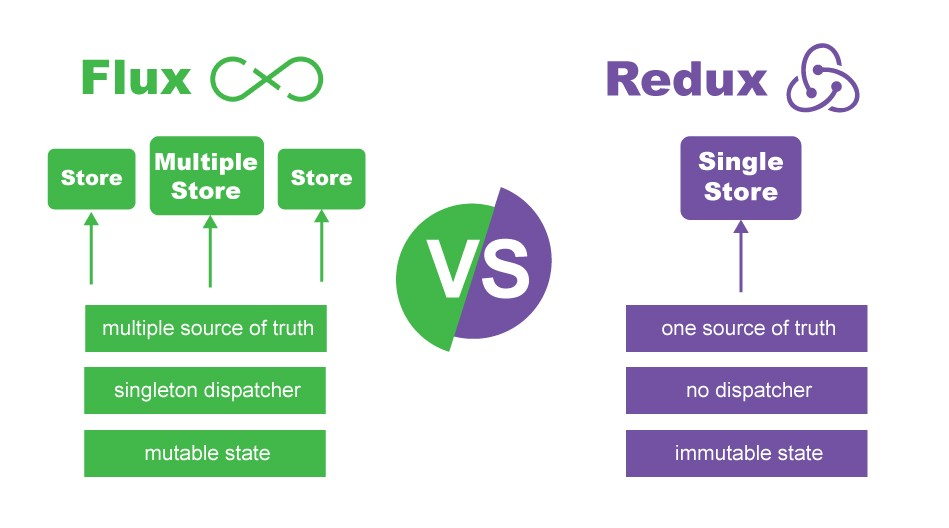
\includegraphics[width=.6\textwidth]{img/reduxFlux}
	\caption{Różnice między Redux a Flux [www.medium.com]}\label{rys:reduxFlux}% Źródło rysunku i etykieta przez którą odwołujemy się do rysunku.
\end{figure}

\subsection{redux-thunk}

Biblioteka \textbf{redux-thunk} została stworzona przez Dana Abramova,
który jednocześnie jest twórcą Reduxa. Pozwala ona tworzyć kreatory akcji,
które zamiast obiektu zwracają funkcję.
Dzięki temu możliwe jest opóźnienie rozgłoszenia akcji lub zgłoszenie jej tylko
jeśli zostaną spełnione określone warunki.~\cite{www_thunk}

Jak dodać thunk do Reduxa pokazuje listing~\ref{listing:thunk-redux}.

\begin{listing}
\begin{minted}{c}
    import { createStore, applyMiddleware } from 'redux';
    import thunk from 'redux-thunk';
    import rootReducer from './reducers/index';

    const store = createStore(
        rootReducer,
        applyMiddleware(thunk)
    );
\end{minted}
\caption{Połączenie Reduxa i Thunka} \label{listing:thunk-redux}
\end{listing}

\begin{center}
	\textbf{Obsługa wywołań asynchronicznych czyli kreatory akcji}
\end{center}

W przykładzie (listing~\ref{listing:firebase_action}) widnieje akcja,
która najpierw dodaje użytkownika do bazy, a następnie rozgłasza akcję dodawania użytkownika,
jeżeli modyfikacja danych w bazie zakończyła się pomyślnie.

W funkcji \texttt{startAddUserToGame} pobierane są najpierw dane o grze, czyli: \texttt{owner},
który jest po prostu identyfikatorem użytkownika Githuba.
Następnie jest pobierany identyfikatory gry \texttt{game}.
Na końcu dostajemy dane użytkownika, którego chcemy dodać do gry.

Funkcja ta zwraca funkcję przyjmującą parametr \texttt{dispatch},
który służy do rozgłaszania danych.
Później jest tworzony użytkownik, który ma zostać dodany do gry (\texttt{tempUser}).
Na końcu jest tworzony obiekt, będący odnośnikiem do użytkowników w bazie,
który pomaga zaktualizować obiekt gry.
Finalnie korzystając z referencji aktualizuje się obiekt gry w bazie danych,
a w razie sukcesu (funkcja \textbf{then}) akcja jest rozsyłana dalej.

\subsection{Połączenie Firebase i Redux}

Jak nie trudno się domyślić, wszystkie operacje pomiędzy Firebase a Redux są realizowane w postaci akcji.
Do synchronizacji frontend i backend służy \textit{Thunk},
który przesyła dane do store’a tylko wtedy,
kiedy nie ma żadnych problemów po stronie Firebase.

Jeżeli baza danych nie będzie mogła pobrać danych bo wystąpił błąd,
Thunk nie wykona żadnych operacji. Sposób połączenia tych dwóch elementów przedstawiono
na rysunku~\ref{rys:fireRedux}.

\begin{figure}
	\centering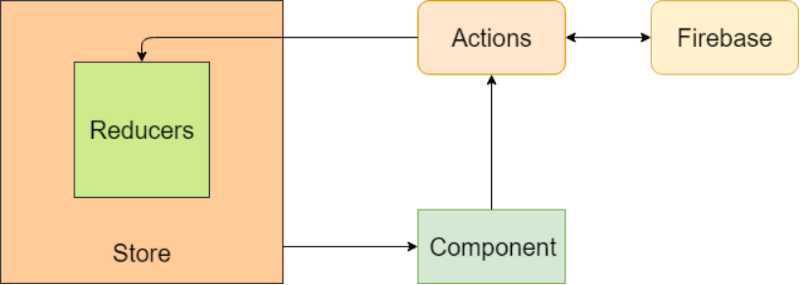
\includegraphics[width=.6\textwidth]{img/fireRedux}
	\caption{Sposób połączenia firebase i reduxa. [medium.com]}\label{rys:fireRedux}% Źródło rysunku i etykieta przez którą odwołujemy się do rysunku.
\end{figure}


% !TeX program = latexmk
% !TeX spellcheck = pl_PL
% !TeX root = example.tex

\chapter{Implementacja projektu}

Aplikacja \textit{Planning Poker}, to aplikacja webowa oparta na platformie Firebase,
która jest napisana przy użyciu biblioteki ReactJS, z wykorzystaniem
edytora Visual Studio Code.

Aby zachować porządek i możliwość późniejszego rozwoju aplikacji o nowe komponenty,
koniecznym jest stworzenie uporządkowanej struktury plików zawartych w projekcie
(rysunek~\ref{rys:projekt}).

\begin{figure}[h]
	\centering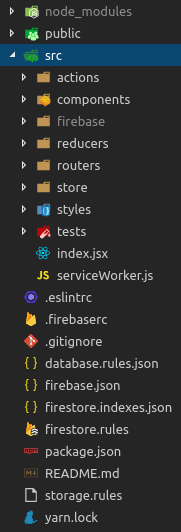
\includegraphics[width=.3\textwidth]{img/projekt.png}
	\caption{Struktura projektu}\label{rys:projekt}% Źródło rysunku i etykieta przez którą odwołujemy się do rysunku.
\end{figure}

Folderem zawierającym wszystkie podfoldery oraz pliki jest folder \texttt{scrumpoker}.
Pliki takie jak \texttt{storage.rules} czy \texttt{.firebaesrc} powstały automatycznie
w procesie konfiguracji usługi Firebase.

Plik \texttt{package.json} zawiera całą konfigurację projektu stworzonego
za pomocą narzędzia \texttt{create-react-app}.

Folder \texttt{node modules} zawiera zależności, niezbędne do uruchomienia aplikacji.

Folder \texttt{src} zawiera cały kod źródłowy aplikacji.
Głównym plikiem projektu jest \texttt{index.jsx}. To w tym pliku renderowana jest cała aplikacja.

Aby uruchomić program,
niezbędny jest też backend w postaci utworzonego i skonfigurowanego projektu Firebase.
Konfiguracje należy umieścić w pliku \texttt{src/firebase/firebase.jsx}
(patrz listing~\ref{listing:firebaseConfig}).

\begin{listing}
\begin{minted}{c}
import * as firebase from 'firebase';

var config = {
    apiKey: "<API_KEY>",
    authDomain: "<PROJECT_ID>.firebaseapp.com",
    databaseURL: "https://<DATABASE_NAME>.firebaseio.com",
    projectId: "<PROJECT_ID>",
    storageBucket: "<BUCKET>.appspot.com",
    messagingSenderId: "<SENDER_ID>",
};

firebase.initializeApp(config);

const database = firebase.firestore();
const settings = { timestampsInSnapshots: true};
database.settings(settings);
export { firebase, database as default };
\end{minted}
\caption{Konfiguracja firebase}\label{listing:firebaseConfig}
\end{listing}

Z wyjątkiem stanu gry, aplikacja wszelkie dane pobiera z serwisu GitHub poprzez
udostępnione API, wykorzystując do tego bibliotekę \texttt{octokit/rest}.

W każdym komponencie, wymagającym danych z tego serwisu,
uruchamiane są metody, które ładują niezbędne dane do stanu komponentu.

Jako że wszelkie gry tworzone w aplikacji dotyczą projektów prowadzonych na GitHub,
użytkownik, aby skorzystać z aplikacji, musi posiadać konto na GitHub oraz co najmniej
jeden projekt założony w tej usłudze.
Biorąc pod uwagę, że w trakcie rozgrywki Planning Pokera oceniane są historyjki z backlog,
użytkownik musi mieć jakieś historyjki przypisane do wybranego projektu w GitHub.
Aby to zrobić, musi utworzyć w projekcie elementy zwane `issues', które w tym momencie traktowane są jako historyjki.
Co za tym idzie, użytkownik musi się zalogować przez serwis GitHub, co ilustruje poniższy rysunek~\ref{rys:login}.

\begin{figure}[h]
	\centering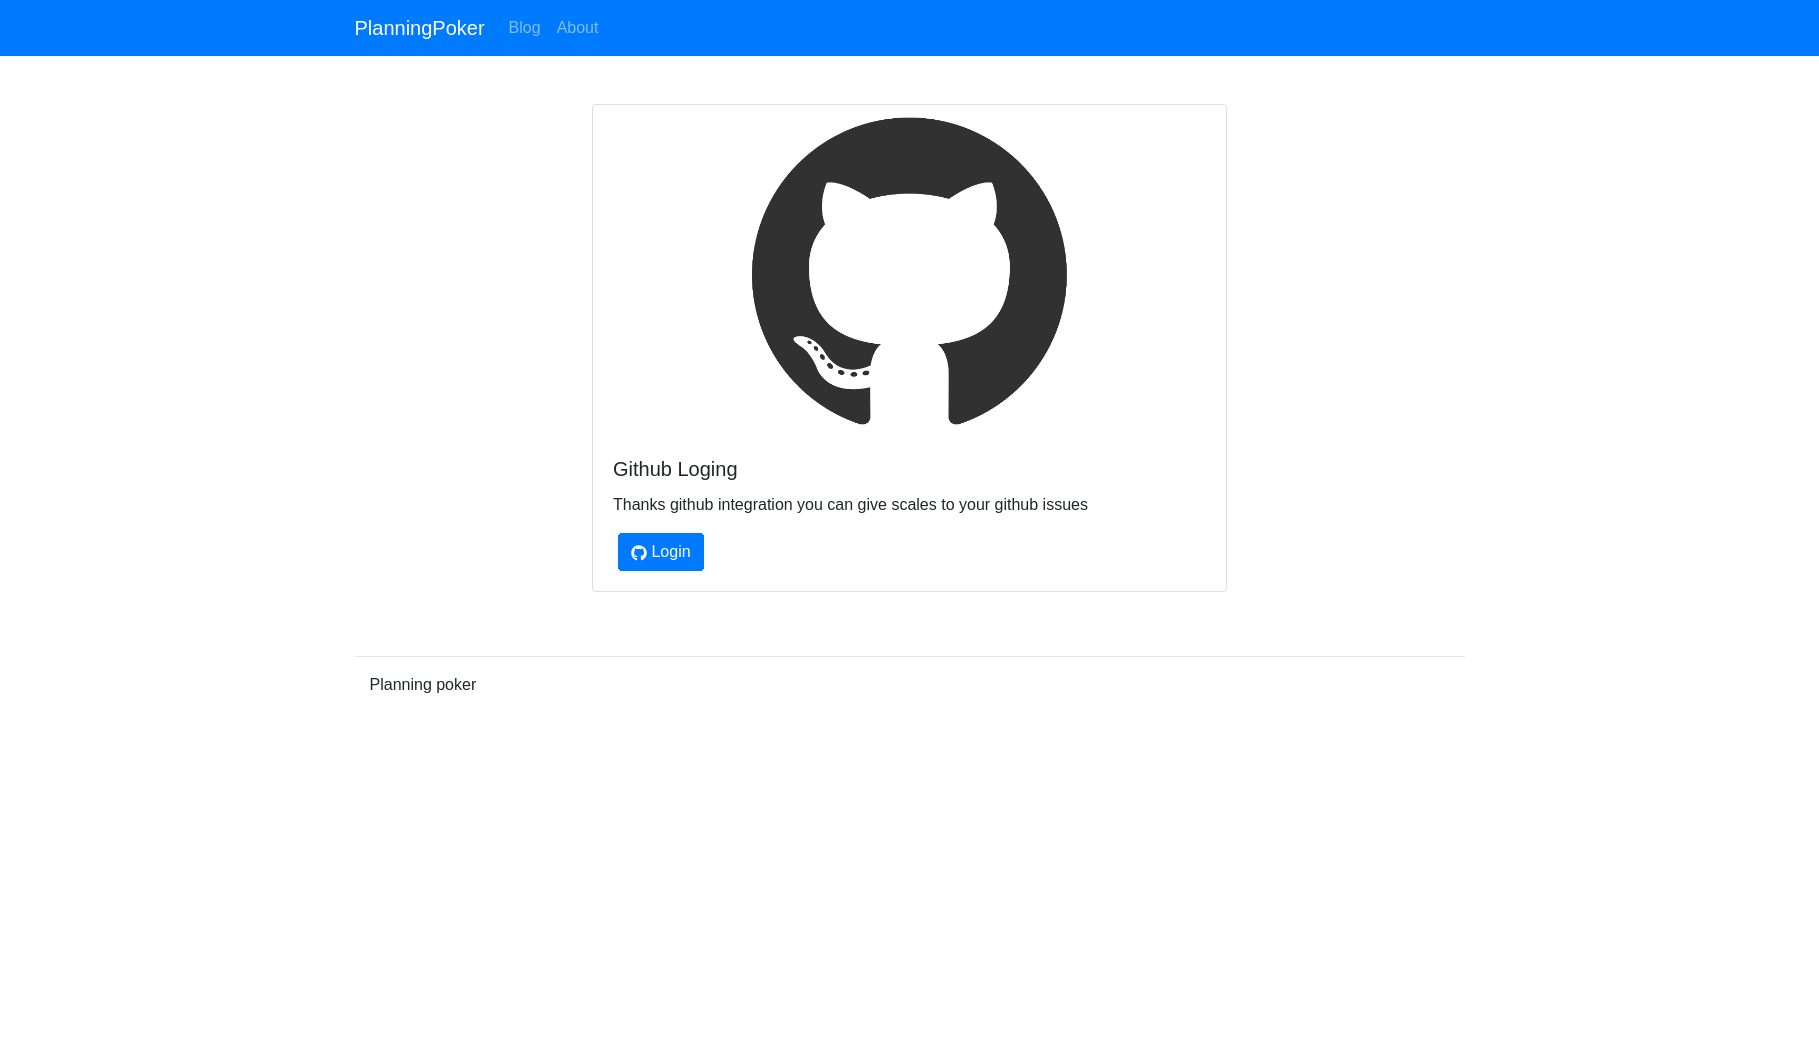
\includegraphics[width=\textwidth]{img/GitLogin.png}
	\caption{Strona logowania}\label{rys:login}% Źródło rysunku i etykieta przez którą odwołujemy się do rysunku.
\end{figure}

\section{Tworzenie gry}

Można założyć, że grupą docelową aplikacji, są użytkownicy GitHub, czyli programiści.
Autor, jako częsty użytkownik tej usługi, odczuł brak aplikacji wspomagającej Planning Poker,
która byłaby z tym narzędziem zintegrowana.

\begin{figure}[h]
	\centering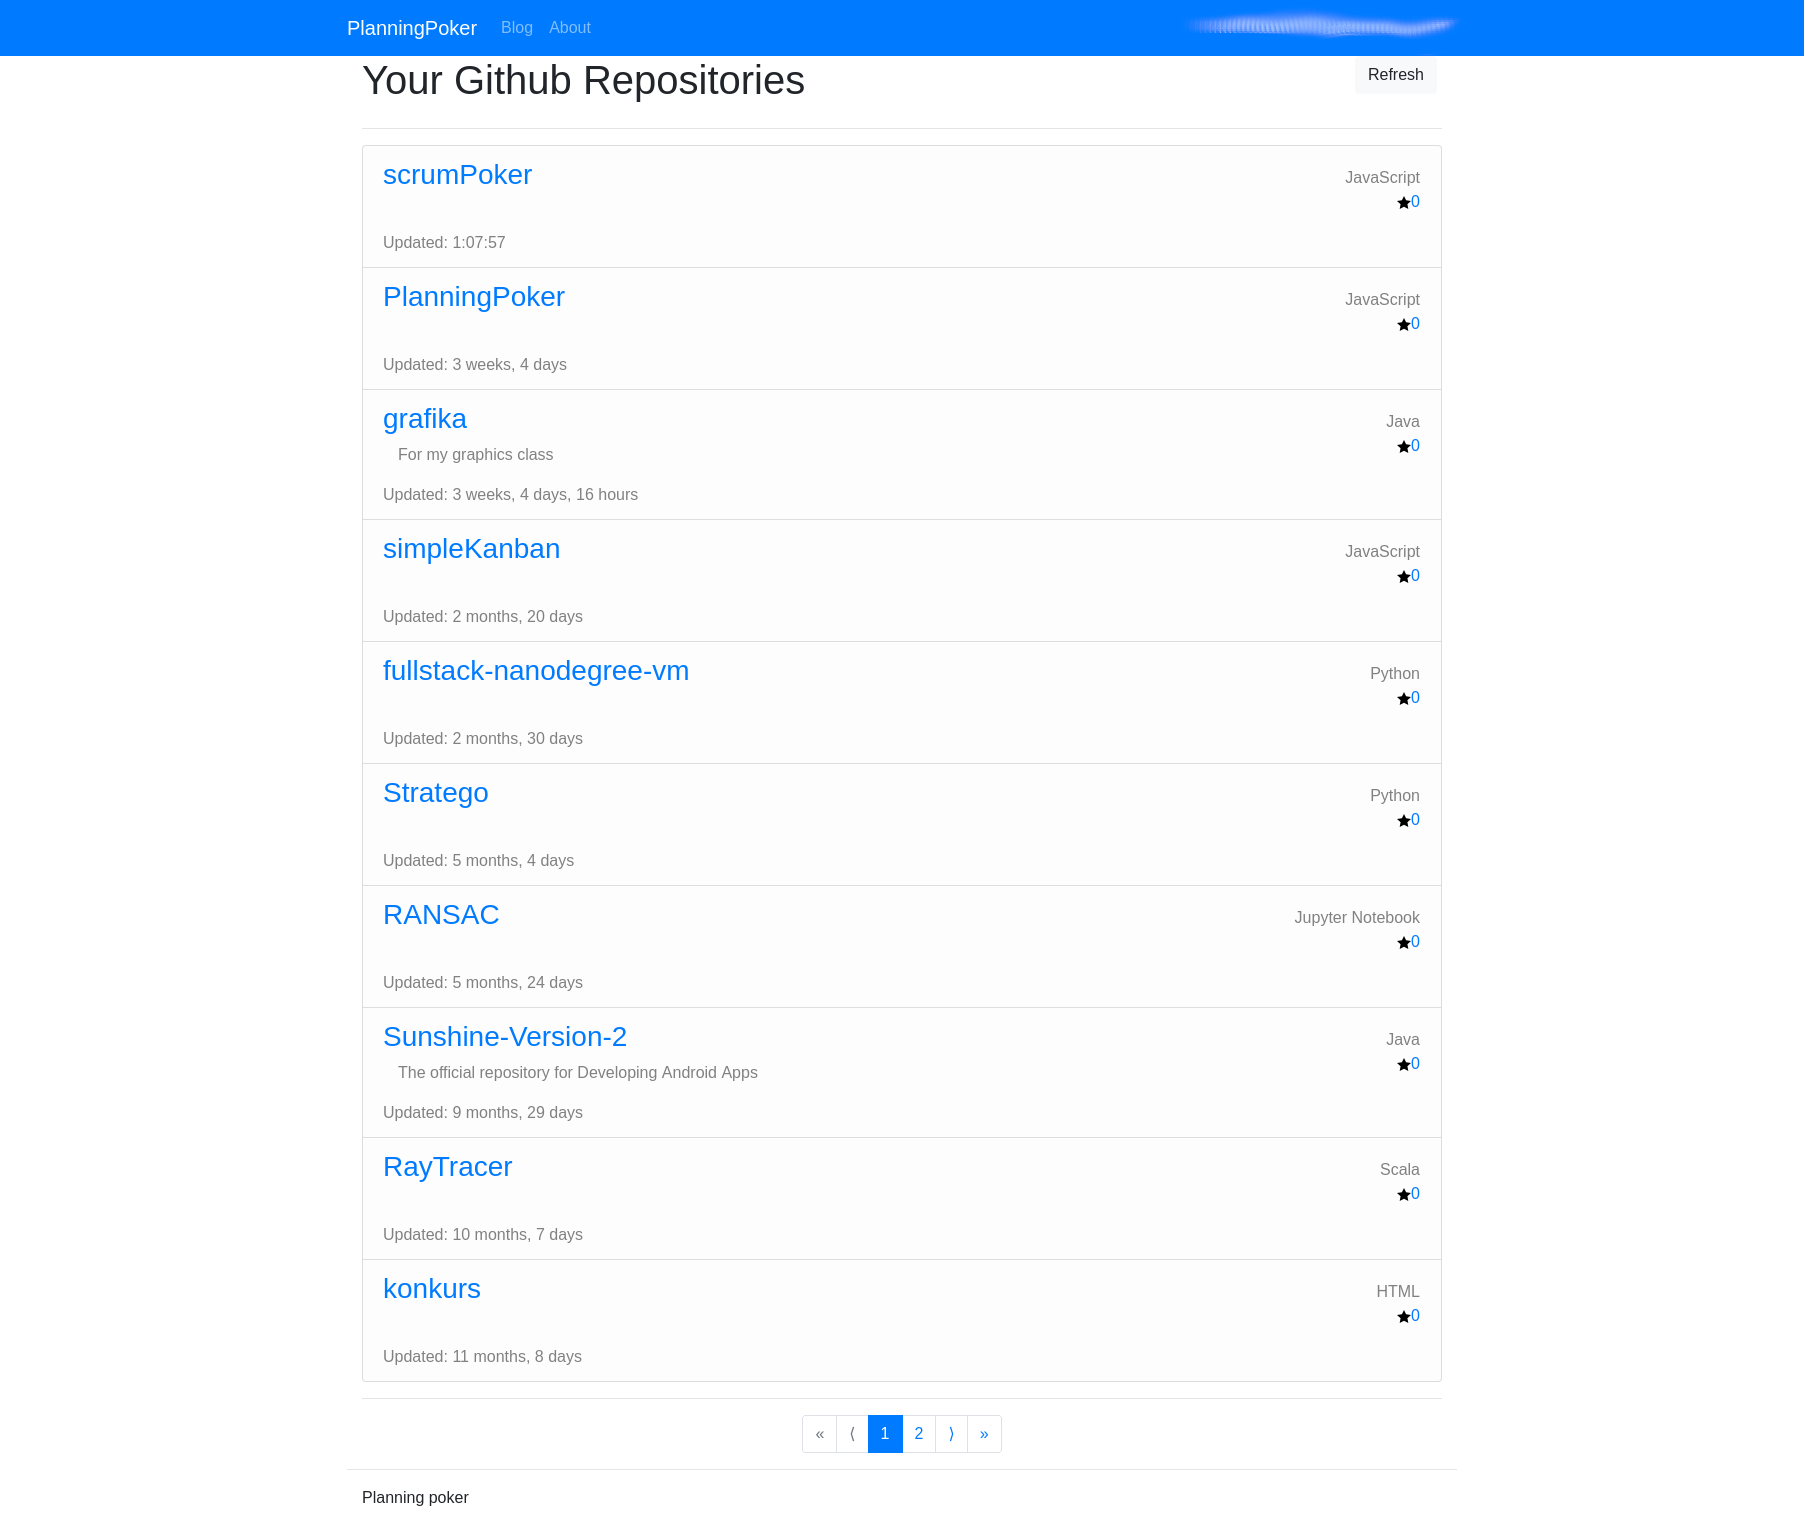
\includegraphics[width=\textwidth]{img/repositories.png}
	\caption{Ekran wyboru projektu}\label{rys:projekty}% Źródło rysunku i etykieta przez którą odwołujemy się do rysunku.
\end{figure}

Autor podczas przeglądania projektów na GitHub zauważył, że jego użytkownicy,
wszelkie problemy czy też propozycje nowych funkcjonalności aplikacji umieszczają
w sekcji \textbf{issues} danego projektu. Stwierdził wówczas, iż aplikacja która ocenia
istniejące problemy lub proponowane cechy, które są dostępne w już sprawdzonym narzędziu
i eksportuje oceny do GitHub w postaci etykiet będzie dobrym pomysłem.


\subsection{Ekran wyboru projektu}

Aby utworzyć grę, najpierw należy wybrać projekt, którego gra będzie dotyczyła.
W aplikacji projektami są repozytoria (rysunek~\ref{rys:projekty}).

\begin{figure}[h]
	\centering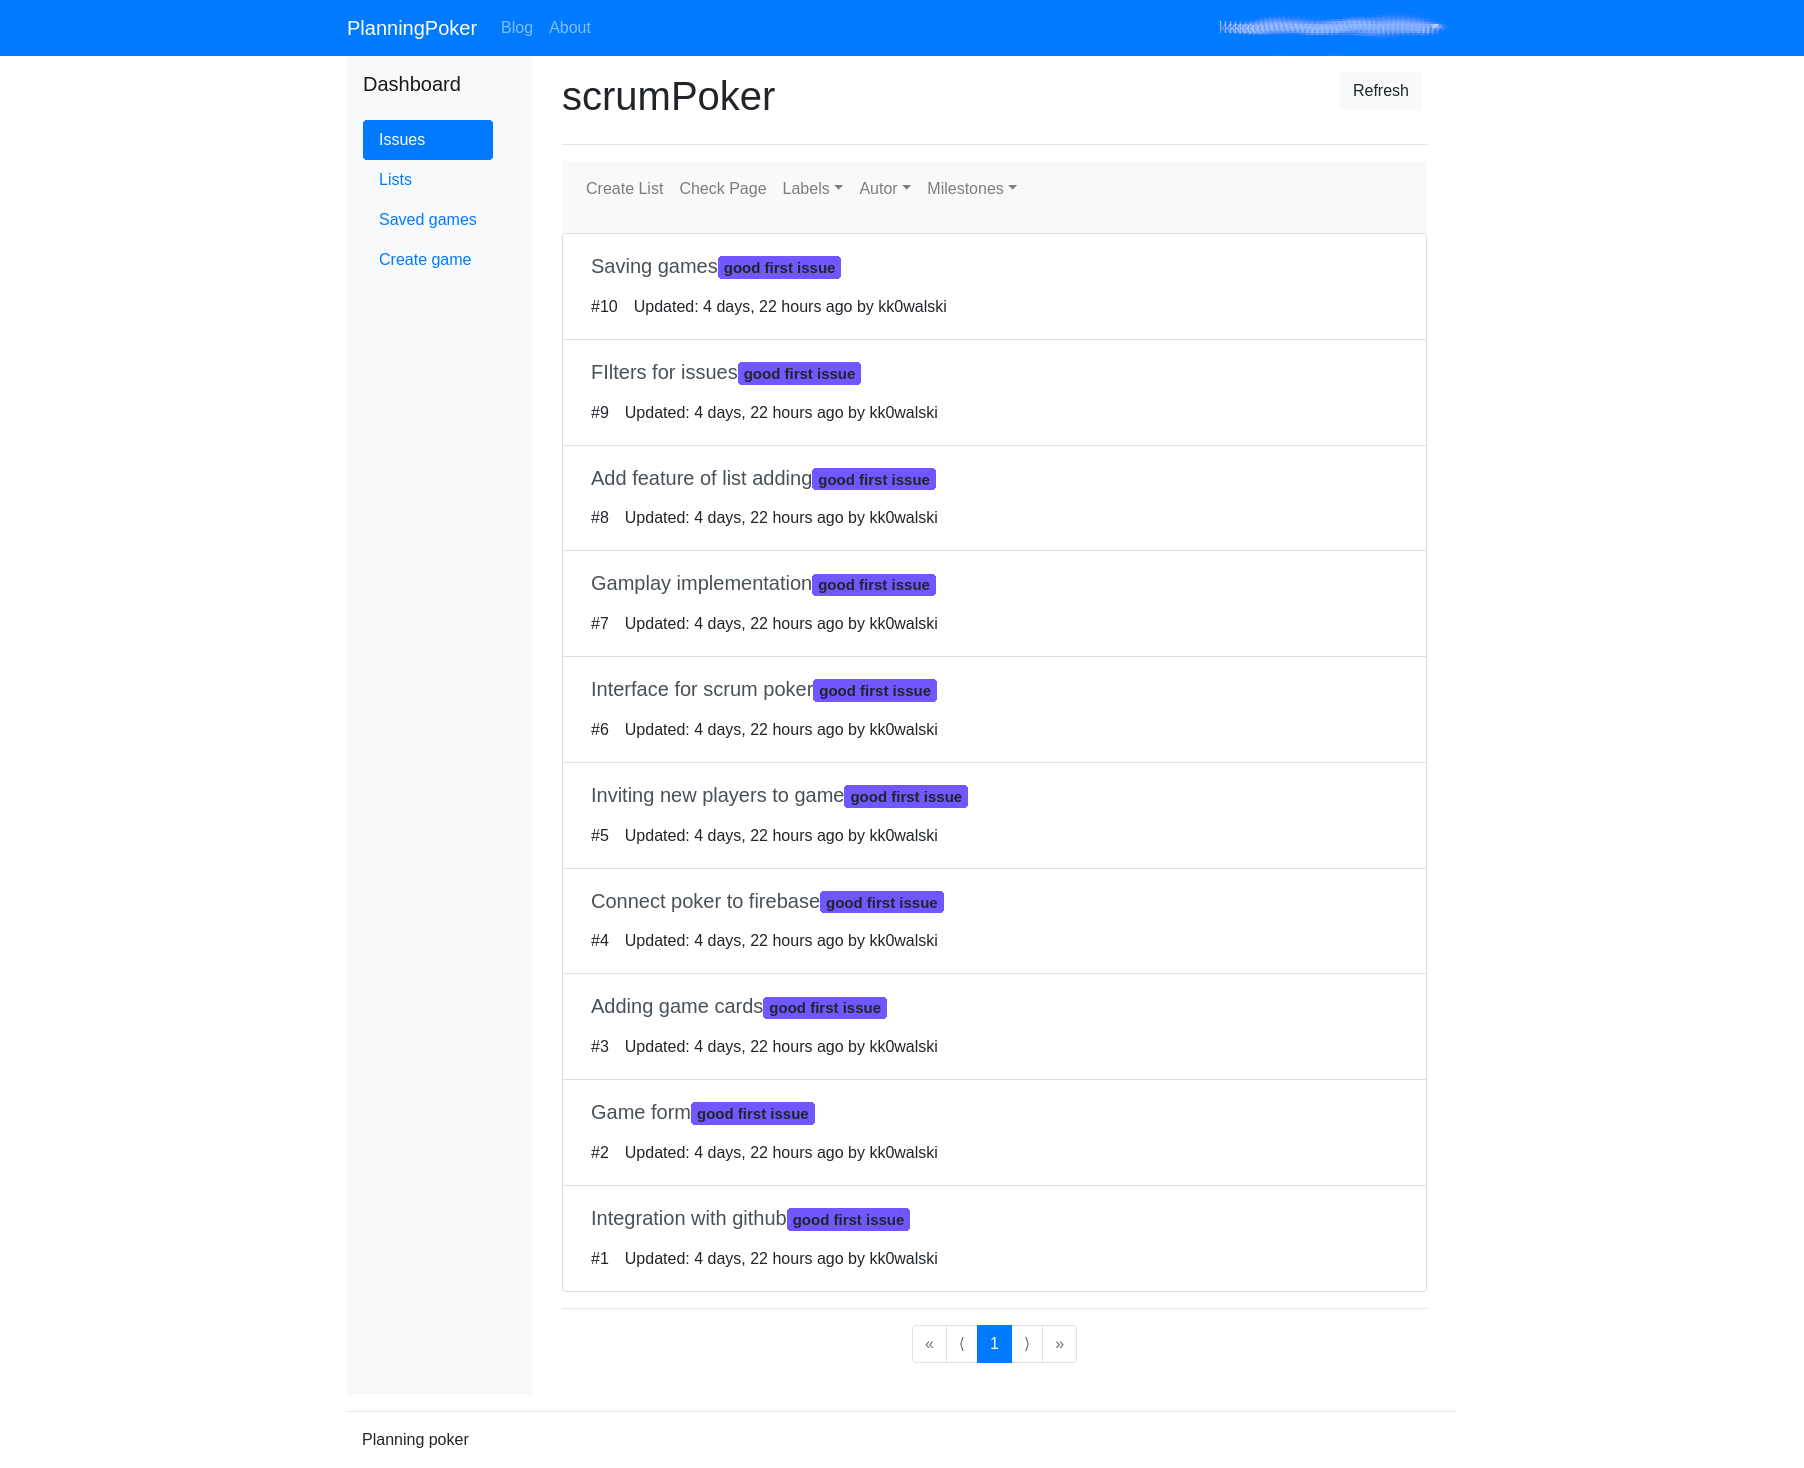
\includegraphics[width=\textwidth]{img/Issues.png}
	\caption{Ekran wyboru backlogu}\label{rys:issues}% Źródło rysunku i etykieta przez którą odwołujemy się do rysunku.
\end{figure}


\subsection{Ekran wyboru backlogu}

Aby rozgrywka miała sens, konieczne jest posiadanie backlogu zadań,
które zespół powinien wyestymować podczas danej sesji planningowej.
Odpowiednią listę zadań tworzy się w panelu ustawień projektu (rysunek~\ref{rys:issues}),
w sekcji \textbf{Issues}.

Dzięki odpowiednim ustawieniom filtrów można odnaleźć elementy po etykietach,
autorze czy po kamieniach milowych.

Aby stworzyć listę, należy wybrać odpowiednie zagadnienia, klikając lewy przycisk myszy,
czy też zaznaczając stronę za pomocą przycisku \textbf{Check page}.

Po wybraniu odpowiednich elementów i naciśnięciu przycisku \textbf{Create List}
pokazywane jest okno potwierdzenia,
które pokazuje wybrane elementy oraz pole do wpisania nazwy listy.

\begin{figure}[h]
	\centering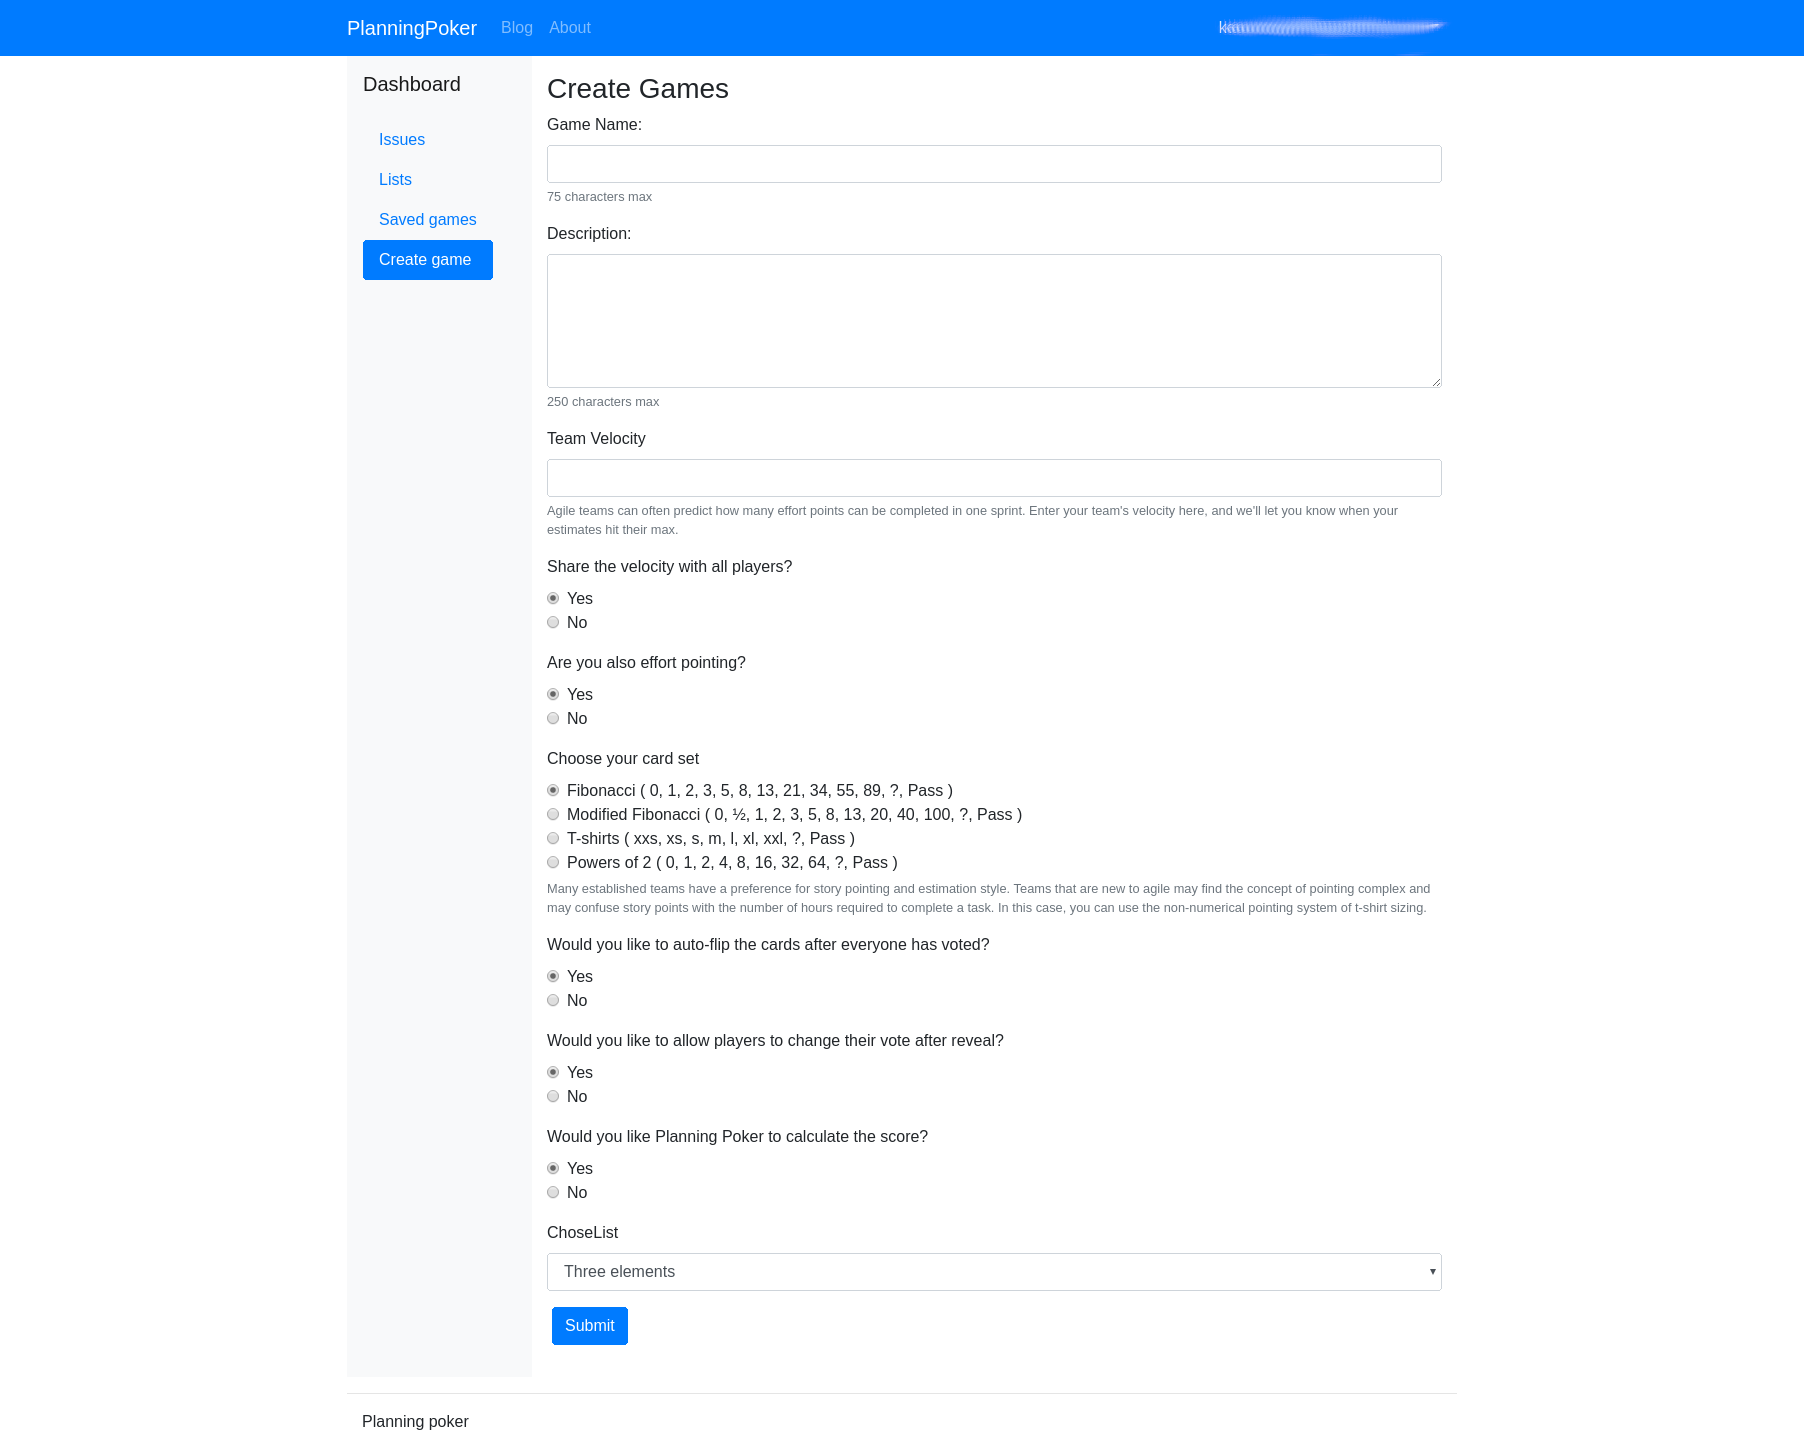
\includegraphics[width=0.8\textwidth]{img/formularz.png}
	\caption{Formularz tworzenia gry}\label{rys:form}% Źródło rysunku i etykieta przez którą odwołujemy się do rysunku.
\end{figure}

Po potwierdzeniu wyboru oraz wpisaniu nazwy listy, jest tworzona lista, zawierająca
identyfikatory wybranych historyjek (czyli \textit{issues} w projekcie GitHub).

Jak zostało już wcześniej wspomniane, niezbędnym elementem gry jest backlog.
Tym backlogiem dla każdej gry będzie lista, którą właściciel tworzy spośród wspomnianych historyjek.
Ta lista będzie później dostępna w formularzu tworzenia gry,
dzięki czemu będzie można ją wybrać przy jej tworzeniu.


\subsection{Ekran ustawień gry}

W trakcie tworzenia gry możemy skorzystać z ekranu ustawień gry (rysunek~\ref{rys:form}),
aby określić jej nazwę i opis ale także parametry, które będą miały wpływ na grę.
Oczywiście, będziemy mogli wybrać skalę estymacji gry, ale także podać prędkość (ang.\ velocity)
naszego zespołu, zdecydować czy inni gracze będą tą prędkość widzieć.
Możemy także zdecydować czy twórca gry również będzie mógł głosować.

Inną ważną kwestią jest to, czy karty powinny być odkrywane, kiedy każdy zagłosował
oraz czy pozwolić graczom zmienić swoją ocenę po pokazaniu wszystkich kart.

Aplikacja może również obliczać wynik punktowy historyjki po zakończonym głosowania automatycznie,
robi to za pomocą średniej ważonej, która później jest zamieniana na najbliższą jej ocenę w skali estymacji.

Na końcu oczywiście należy wybrać backlog w postaci odpowiedniej listy, tu należy zaznaczyć,
że jeżeli w projekcie nie będzie stworzonej żadnej listy, to nie będzie można stworzyć gry.

Pewne ustawienia gry można zmienić także już po jej utworzeniu.

\section{Rozgrywka}

Do rozgrywki Planning Pokera oczywiście potrzebni są gracze.
Aby rozgrywka była możliwa dla więcej niż jednego gracza, konieczna jest komunikacja z serwerem.
Wszelkie akcje podczas gry są synchronizowane za pomocą Firebase,
a dzięki odpowiednim słuchaczom aplikacja reaguje na wszelkie zmiany w stanie gry.

Gracz jest dodawany do gry poprzez udostępnianie innym użytkownikom odnośnika do gry
w postaci jej adresu URL\@.
Jeżeli gracz wejdzie do gry, zostanie poproszony o podanie nazwy,
dzięki której będzie można go odróżnić od innych graczy.
Gracze są dodawani do bazy danych dzięki funkcji usługi Firebase nazwanej „anonimowe logowanie”.
Gracze w grze mogą tylko i wyłącznie głosować,
natomiast właściciel gry wybiera historyjkę do głosowania, to znaczy że to on narzuca tempo gry.
Panel gry pokazuje rysunek~\ref{rys:gra}.

\begin{figure}[h]
	\centering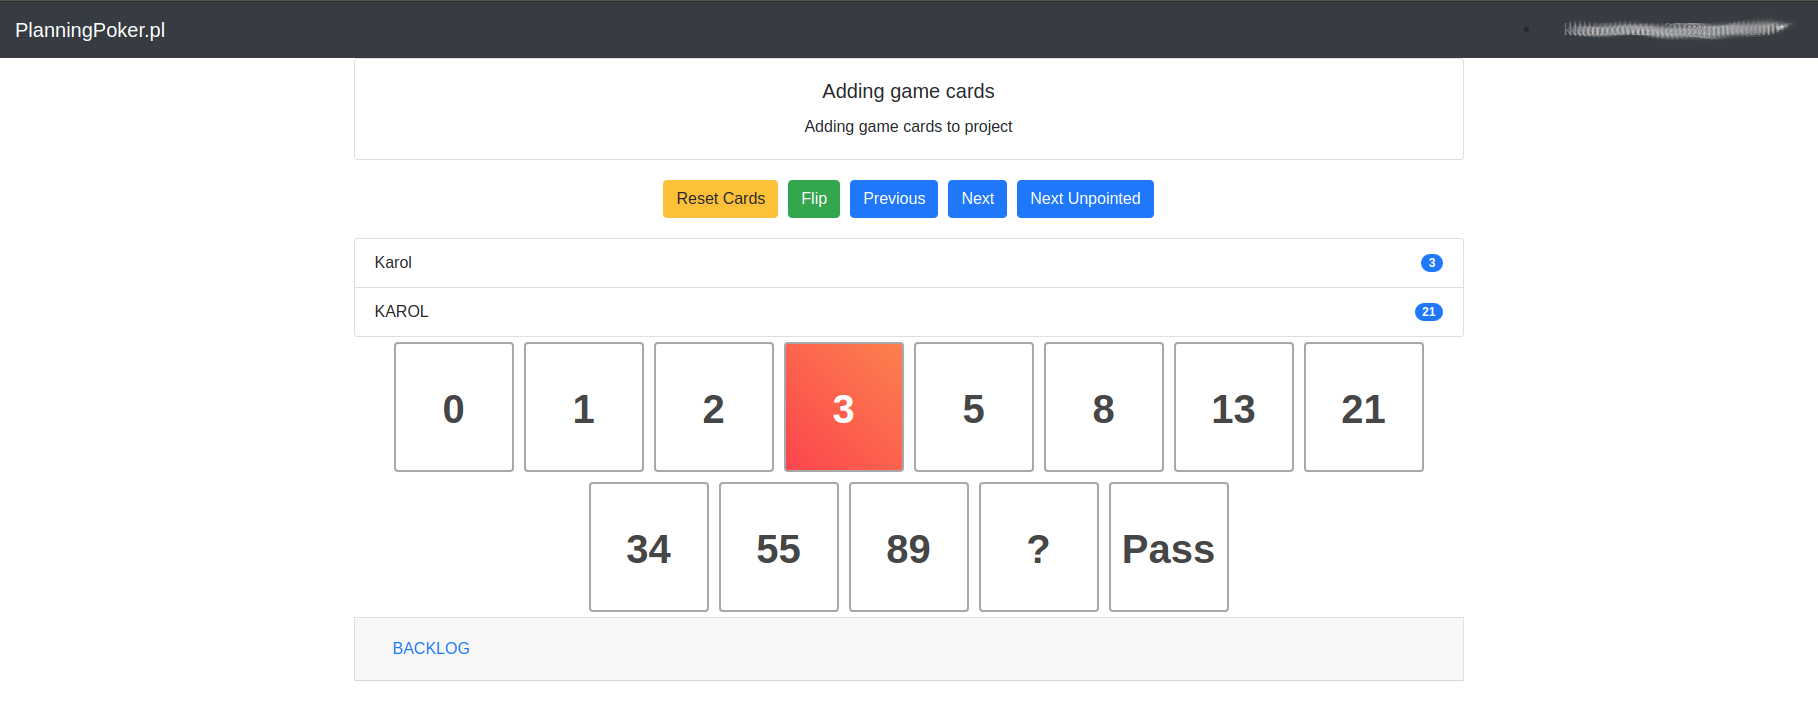
\includegraphics[width=\textwidth]{img/gra.png}
	\caption{Panel gry}\label{rys:gra}% Źródło rysunku i etykieta przez którą odwołujemy się do rysunku.
\end{figure}

\section{Komunikacja słowna}

Istotnym elementem każdego Planning Pokera jest komunikacja między graczami,
autor jednak stwierdził,
iż na rynku istnieją już odpowiednie aplikacje do komunikacji,
a firmy produkujące oprogramowanie mają preferowane komunikatory, których używają
również w innych sytuacjach niż proces planowania sprintu.
A więc przed każdą rozgrywką autor poleca wybrać odpowiedni komunikator do komunikacji w trakcie gry.


\section{Wynik implementacji}

Nie wszystkie zaplanowane elementy znajdują się w aplikacji,
jednak najważniejsze funkcjonalności zostały zaimplementowane:

 \begin{itemize}
	\item Logowanie przez GitHub
	\item Pobieranie Issues z GitHub
	\item Tworzenie list, które będą backlog'iem w grze
	\item Tworzenie gier
	\item Rozgrywka
	\item Eksport wyników gier do GitHub
	\item Możliwość usunięcia gry
	\item Możliwość zmiany ustawień gry
	\item Możliwość zapraszania użytkowników do gry
\end{itemize}

Funkcje których nie udało się zaimplementować to:

\begin{itemize}
	\item Pełna synchronizacja z GitHub
	\item Edycja historyjek wraz z synchronizacją zmian z GitHub
	\item Możliwość usuwania użytkownika z gry
\end{itemize}

\section{Podsumowanie}

Dzięki użyciu odpowiednich technologii udało się stworzyć w pełni funkcjonalną aplikację,
umożliwiającą zespołom zdalnym przeprowadzenie sesji planningowej nad dobrze
zdefiniowanym backlogiem zadań.
Nie znaczy to jednak, że jej stworzenie było proste.
Autorowi zajęło sporo czasu wybranie odpowiednich technologii do projektu.
Można powiedzieć że niniejsza praca była świetną okazją do poznania
wielu nowych narzędzi do tworzenia aplikacji internetowych wykorzystujących
komunikację w czasie rzeczywistym.



\chapter{Ewaluacja aplikacji}

W Słowniku Języka Polskiego PWN znajdziemy następujące hasło: \begin{quote}
    \textls{„ewaluacja – ustalenie wartości i ceny czegoś, ocenianie, oszacowanie”. }
\end{quote}
Ewaluacja to słowo pochodzące z języka francuskiego oznaczające oszacowanie lub określenie wartości, czasem również ocenę. Takie znaczenie ma też w literaturze anglojęzycznej. Pojęcie to również w Polsce nie jest niczym nowym, gdyż w 1929 roku słownik M. Arcta mówi o niej: „ocenianie, oszacowanie, określenie wartości”. „Proces zmierzający do stwierdzenia, w jakim stopniu założone cele są rzeczywiście realizowane” (R. W. Tyler). Ze względu na kryterium czasu, może to być:
\begin{itemize}
    \item ewaluacja wstępna / szacunkowa,
    \item ewaluacja ad hoc / bieżąca lub ciągła,
    \item ewaluacja ex-post / końcowa.
\end{itemize}
W naszym przypadku, z uwagi na to, że aplikacja jest już gotowa, będzie to ewaluacja „ex-post”. \newline
Ze względu na sposób prowadzenia badania rozróżniamy:
\begin{itemize}
    \item ewaluacje wewnętrzne
    \item ewaluacje zewnętrzne
\end{itemize}

\section{Plan badania}
Zastosowano ewaluację zewnętrzną, czyli powołano dwa pięcioosobowe zespoły projektowe z
jednej z zaprzyjaźnionych wrocławskich firm informatycznych, które wykorzystały naszą aplikację do
przeprowadzenia dwóch rozgrywek Planning Pokera, w celu estymacji zestawu historyjek stworzonych dla
celów testowych tylko dla tego projektu. Jeden zespól spotkał się w siedzibie firmy w sali konferencyjnej,
natomiast drugi zespól przeprowadził rozgrywkę zdalnie korzystając z komunikatora internetowego Microsoft
Lync. Oba zespoły w celu przeprowadzenia rozgrywki korzystały z naszej aplikacji.
\section{Metoda badania}
Po zakończeniu obu rozgrywek poproszono uczestników o wypełnienie stosownych ankiet.
Ankiety zostały opracowane zgodnie ze Skalą Użyteczności Systemu (System Usability Scale, SUS).
Skala ta została wymyślona przez Johna Brooke'a, który w 1986 roku stworzył szybką skalę użyteczności, aby
ocenić praktycznie każdy rodzaj systemu. \newline
SUS został wypróbowany i przetestowany przez prawie 30 lat użytkowania i sprawdził się jako
niezawodna metoda oceny użyteczności systemów w porównaniu do standardów branżowych. \newline
SUS składa się 10 pytań oraz 5 stopniowej skali ocen (opartej o skalę Likerta):
\begin{enumerate}
    \item Będę często korzystał z systemu.
    \item System jest niepotrzebnie skomplikowany.
    \item System jest łatwy w użyciu.
    \item Będę potrzebował wparcia technicznego, aby korzystać z systemu.
    \item Różne funkcje systemu są łatwo dostępne.
    \item W systemie jest zbyt wiele niespójności.
    \item Większość osób będzie w stanie opanować system bardzo szybko.
    \item System jest kłopotliwy w użyciu.
    \item Czuję się bardzo pewnie korzystając z systemu.
    \item Musiałem opanować wiele rzeczy przed rozpoczęciem pracy z systemem.
\end{enumerate}

\subsection{Jak obliczyć SUS}
Po zebraniu wyników przechodzimy do kolejnego kroku, w którym obliczamy wskaźnik SUS. Wynik
testu określany jest w punktach na skali od 0 do 100. \newline
Krok 1. Przyporządkowujemy do każdej odpowiedzi wartości od 0 do 4, zgodnie ze schematem podanym
poniżej. \newline
\newline
dla pytań 1, 3, 5, 7, 9 należy przypisać następującą punktację :
\begin{itemize}
    \item Zdecydowanie nie zgadzam się = 0
    \item Raczej nie zgadam się = 1
    \item Nie mam zdania = 2
    \item Raczej zgadzam się = 3
    \item Zdecydowanie zgadzam się = 4
\end{itemize}
dla pytań 2, 4, 6, 8, 10 punktacja wygląda następująco :
\begin{itemize}
    \item Zdecydowanie nie zgadzam się = 4
    \item Raczej nie zgadam się = 3
    \item Nie mam zdania = 2
    \item Raczej zgadzam się = 1
    \item Zdecydowanie zgadzam się = 0
\end{itemize}
Krok 2. Sumujemy punkty i mnożymy otrzymaną wartość przez 2.5.
Wynik powinien mieścić się w przedziale 0 - 100.
\subsection{Jak interpretować SUS}
Im większy wynik tym lepsza użyteczność. Wartości powyżej 68 są interpretowane jako dobry wynik,
natomiast wynik równy lub większy od 80,3 to wynik bardzo dobry. Z kolei wynik 51 lub niższy oznacza, że
użyteczność aplikacji jest niewystarczająca i koniecznie trzeba nad nią popracować. \cite{www_SUS}
\section{Wyniki testów}
Wyniki przeprowadzonych ankiet przedstawione zostały w tabelach \ref{tabela:badanie1} i \ref{tabela:badanie2} - jedna dotyczy zespołu,
który zebrał się w sali konferencyjnej, druga dotyczy zespołu wirtualnego (zdalnego).
Przyglądając się wynikom ankiet wg. System Usability Scale (SUS), można zauważyć, że zespól zdalny
ocenił aplikację nieco gorzej, bo na 77 punktów tab:\ref{tabela:badanie2}, natomiast zespół „bliski” na 83,5 punktów. Daje to
średni wynik 80,25, czyli prawie 80,3. Tab: \ref{tabela:badanie1}
Można powiedzieć, że w tym szybkim badaniu osiągnęliśmy wynik bardzo dobry. Warto jednak
bardziej szczegółowo przeanalizować wyniki ankiet. Można zauważyć, że zarówno jeden, jak i drugi
zespół projektowy przyznał mniej punktów odpowiadając na pytania 2, 6 i 8:
\begin{itemize}
    \item 2. System jest niepotrzebnie skomplikowany.
    \item 6. W systemie jest zbyt wiele niespójności.
    \item 8. System jest kłopotliwy w użyciu
\end{itemize}
\begin{landscape}
    \begin{table}
        \centering\caption{Tablica wyników ankiet SUS dla zespołu „bliskiego”\label{tabela:badanie1}}
        \begin{tabular}{|l|l|c|c|c|c|c|c|c|c|c|c|l|}
            \hline
             & Ocena & Q1  & Q2  & Q3  & Q4  & Q5  & Q6  & Q7  & Q8  & Q9  & Q10 & Suma*2.5\\
            \hline
            \multirow{5}{*}{
                \rotatebox{90}{USER1}
            }
             & Zdecydowanie zgadzam się &     &     &     &     &     &     &     &     &     & 4   & \multirow{5}{*}{82.5} \\ \cline{2-12}
             & Raczej nie zgadzam się   &     & 3   &     & 3   &     & 3   &     &     &     &     &                       \\ \cline{2-12}
             & Nie mam zdania           &     &     &     &     &     &     &     & 2   &     &     &                       \\ \cline{2-12}
             & Raczej zgadzam się       &     &     &     &     & 3   &     &     &     &     &     &                       \\ \cline{2-12}
             & Zdecydowanie zgadzam się & 4   &     & 4   &     &     & 4   &     &     &     &     &                       \\ 
            \hline
            \multirow{5}{*}{
                \rotatebox{90}{USER2}
            }
             & Zdecydowanie zgadzam się &     &     &     & 4   &     &     &     &     &     & 4   & \multirow{5}{*}{87.5} \\ \cline{2-12}
             & Raczej nie zgadzam się   &     &     &     &     &     & 3   &     &     &     &     &                       \\ \cline{2-12}
             & Nie mam zdania           &     & 2   &     &     &     &     &     & 2   &     &     &                       \\ \cline{2-12}
             & Raczej zgadzam się       &     &     &     &     &     &     &     &     &     &     &                       \\ \cline{2-12}
             & Zdecydowanie zgadzam się & 4   &     & 4   &     & 4   &     & 4   &     & 4   &     &                       \\
            \hline
            \multirow{5}{*}{
                \rotatebox{90}{USER3}
            }
             & Zdecydowanie zgadzam się &     &     &     &     &     &     &     &     &     & 4   & \multirow{5}{*}{80}   \\ \cline{2-12}
             & Raczej nie zgadzam się   &     & 3   &     & 3   &     &     &     & 3   &     &     &                       \\ \cline{2-12}
             & Nie mam zdania           &     &     &     &     &     & 2   &     &     &     &     &                       \\ \cline{2-12}
             & Raczej zgadzam się       &     &     & 3   &     & 3   &     &     &     & 3   &     &                       \\ \cline{2-12}
             & Zdecydowanie zgadzam się & 4   &     &     &     &     &     & 4   &     &     &     &                       \\
            \hline
            \multirow{5}{*}{
                \rotatebox{90}{USER4}
            }
             & Zdecydowanie zgadzam się &     &     &     & 4   &     &     &     &     &     & 4   & \multirow{5}{*}{82.5} \\ \cline{2-12}
             & Raczej nie zgadzam się   &     &     &     &     &     &     &     & 3   &     &     &                       \\ \cline{2-12}
             & Nie mam zdania           &     & 2   &     &     &     & 2   &     &     &     &     &                       \\ \cline{2-12}
             & Raczej zgadzam się       & 3   &     & 3   &     &     &     &     &     &     &     &                       \\ \cline{2-12}
             & Zdecydowanie zgadzam się &     &     &     &     & 4   &     & 4   &     &     &     &                       \\
            \hline
            \multirow{5}{*}{
                \rotatebox{90}{USER5}
            }
             & Zdecydowanie zgadzam się &     &     &     &     &     &     &     &     &     & 4   & \multirow{5}{*}{85}   \\ \cline{2-12}
             & Raczej nie zgadzam się   &     & 3   &     & 3   &     & 3   &     & 3   &     &     &                       \\ \cline{2-12}
             & Nie mam zdania           &     &     &     &     &     &     &     &     &     &     &                       \\ \cline{2-12}
             & Raczej zgadzam się       & 3   &     &     &     &     &     & 3   &     &     &     &                       \\ \cline{2-12}
             & Zdecydowanie zgadzam się &     &     & 4   &     & 4   &     &     &     & 4   &     &                       \\
            \hline
             & Średnia                  & 3.6 & 2.6 & 3.6 & 3.4 & 3.6 & 2.6 & 3.8 & 2.5 & 3.6 & 4   & 83.5                  \\
            \hline
        \end{tabular}
    \end{table}
\end{landscape}
\begin{landscape} 
    \begin{table}
        \centering\caption{Tablica wyników ankiet SUS dla zespołu zdalnego.\label{tabela:badanie2}}
        \begin{tabular}{|l|l|c|c|c|c|c|c|c|c|c|c|l|}
            \hline
             & Ocena & Q1  & Q2  & Q3  & Q4  & Q5  & Q6  & Q7  & Q8  & Q9  & Q10 & Suma*2.5\\
            \hline
            \multirow{5}{*}{
                \rotatebox{90}{USER1}
            }
             & Zdecydowanie zgadzam się &     &     &     & 4   &     &     &     &     &     & 4   & \multirow{5}{*}{80}   \\ \cline{2-12}
             & Raczej nie zgadzam się   &     &     &     &     &     &     &     & 3   &     &     &                       \\ \cline{2-12}
             & Nie mam zdania           &     &     &     &     &     &     & 2   &     &     &     &                       \\ \cline{2-12}
             & Raczej zgadzam się       & 3   &     & 3   &     &     &     & 3   &     &     &     &                       \\ \cline{2-12}
             & Zdecydowanie zgadzam się &     &     &     &     & 4   &     &     &     & 4   &     &                       \\ 
            \hline
            \multirow{5}{*}{
                \rotatebox{90}{USER2}
            }
             & Zdecydowanie zgadzam się &     &     &     &     &     &     &     &     &     & 4   & \multirow{5}{*}{77.5} \\ \cline{2-12}
             & Raczej nie zgadzam się   &     &     &     & 3   &     & 3   &     &     &     &     &                       \\ \cline{2-12}
             & Nie mam zdania           &     & 2   &     &     &     &     &     & 2   &     &     &                       \\ \cline{2-12}
             & Raczej zgadzam się       &     &     & 3   &     & 3   &     &     &     & 3   &     &                       \\ \cline{2-12}
             & Zdecydowanie zgadzam się & 4   &     &     &     &     &     & 4   &     &     &     &                       \\
            \hline
            \multirow{5}{*}{
                \rotatebox{90}{USER3}
            }
             & Zdecydowanie zgadzam się &     &     &     &     &     &     &     &     &     & 4   & \multirow{5}{*}{82.5} \\ \cline{2-12}
             & Raczej nie zgadzam się   &     &     &     & 3   &     &     &     & 3   &     &     &                       \\ \cline{2-12}
             & Nie mam zdania           &     & 2   &     &     &     & 2   &     &     &     &     &                       \\ \cline{2-12}
             & Raczej zgadzam się       &     &     &     &     &     &     & 3   &     &     &     &                       \\ \cline{2-12}
             & Zdecydowanie zgadzam się & 4   &     & 4   &     & 4   &     &     &     & 4   &     &                       \\
            \hline
            \multirow{5}{*}{
                \rotatebox{90}{USER4}
            }
             & Zdecydowanie zgadzam się &     &     &     &     &     &     &     &     &     &     & \multirow{5}{*}{70}   \\ \cline{2-12}
             & Raczej nie zgadzam się   &     &     &     & 3   &     &     &     &     &     & 3   &                       \\ \cline{2-12}
             & Nie mam zdania           & 2   & 2   &     &     &     & 2   &     & 2   &     &     &                       \\ \cline{2-12}
             & Raczej zgadzam się       &     &     &     &     & 3   &     &     &     & 3   &     &                       \\ \cline{2-12}
             & Zdecydowanie zgadzam się &     &     & 4   &     &     &     & 4   &     &     &     &                       \\
            \hline
            \multirow{5}{*}{
                \rotatebox{90}{USER5}
            }
             & Zdecydowanie zgadzam się &     &     &     &     &     &     &     &     &     & 4   & \multirow{5}{*}{75}   \\ \cline{2-12}
             & Raczej nie zgadzam się   &     & 3   &     & 3   &     &     &     & 3   &     &     &                       \\ \cline{2-12}
             & Nie mam zdania           &     &     &     &     &     & 2   &     &     &     &     &                       \\ \cline{2-12}
             & Raczej zgadzam się       & 3   &     & 3   &     & 3   &     & 3   &     & 3   &     &                       \\ \cline{2-12}
             & Zdecydowanie zgadzam się &     &     &     &     &     &     &     &     &     &     &                       \\
            \hline
             & Średnia                  & 3.2 & 2.2 & 3.4 & 3.2 & 3.4 & 2.2 & 3.4 & 2.6 & 3.4 & 3.8 & 77                    \\
            \hline
        \end{tabular}
    \end{table}
\end{landscape}
Znalazło to potwierdzenie w rozmowie z uczestnikami badania, którzy podnosili następujące kwestie:
\begin{itemize}
    \item Niezbyt wygodny ekran, ponieważ wymaga skrolowania.
    \item Niespójny interfejs.
    \item Zbyt dużo kroków do rozpoczęcia nowej gry.
    \item Nie można stworzyć backloga do gry za pomocą tekstowego filtra.
    \item Brak szczegółowej instrukcji.
    \item Brak pomocy.
\end{itemize}
Badani stwierdzili, iż aplikacja spełnia założony cel. Wymaga ona jeszcze dopracowania. Jednak dzięki
swoim unikatowym cechom może znaleźć grupę docelową.
Zespół zaznaczył, że w sposób podobny oceniają swoje historyjki w postaci etykiet na GitHub, jednak
robią to ręcznie. Głosowanie odbywa się wtedy przy użyciu komunikatora, jednak jest to bardzo czasochłonne i
zdarzają się problemy. Uczestnicy badania stwierdzili, że takie narzędzie z pewnością ułatwiłoby im estymacje.
Po wynikach ankiet widać, że aplikacja wymaga jeszcze dopracowania. Problemem jest nawigacja po
aplikacji, gdyż wymaga zbyt wielu przejść do ekranów by rozpocząć grę. Członkowie najchętniej zaczęliby grę,
wpisując w pole tekstowe nazwę repozytorium, a w drugie odpowiednie filtry by zacząć grę. W aplikacji nie ma
też zbyt wielu przydatnych objaśnień. Według jednego z programistów sam formularz ustawień gry powinien
być trochę przeprojektowany, aby wiadomo było, jakie pola są obowiązkowe, oraz co zmieniają w całej
rozgrywce.
Aplikacji przydałby się też odpowiedni dział pomocy, mówiący o tym jak grać w Planning Poker, oraz jak
należy odpowiednio estymować zadania. Mimo tego aplikacja dzięki swojej integracji z narzędziem GitHub
wyróżnia się na tle konkurencji. Jeżeli w aplikacji zostanie przeprojektowany sposób tworzenia gry na szybszy
oraz dodane trochę więcej opcji to może okazać się dość dobrym wyborem dla programistów.
Można przyznać, iż aplikacja spełnia swoje zadanie i z powodzeniem może być wykorzystana jako
narzędzie wspomagające estymację zadań projektowych metodą Planning Poker.


\chapter*{Zakończenie}

W pracy udało mi się dużo zrobić. \lipsum[17]

Mnóstwo innych rzeczy da się poprawić i rozwinąć. \lipsum[23]

\appendixpage
\appendix
%\addappheadtotoc

\chapter{Ankieta ekspercka}\label{Dod1}

\begin{figure}
	\centering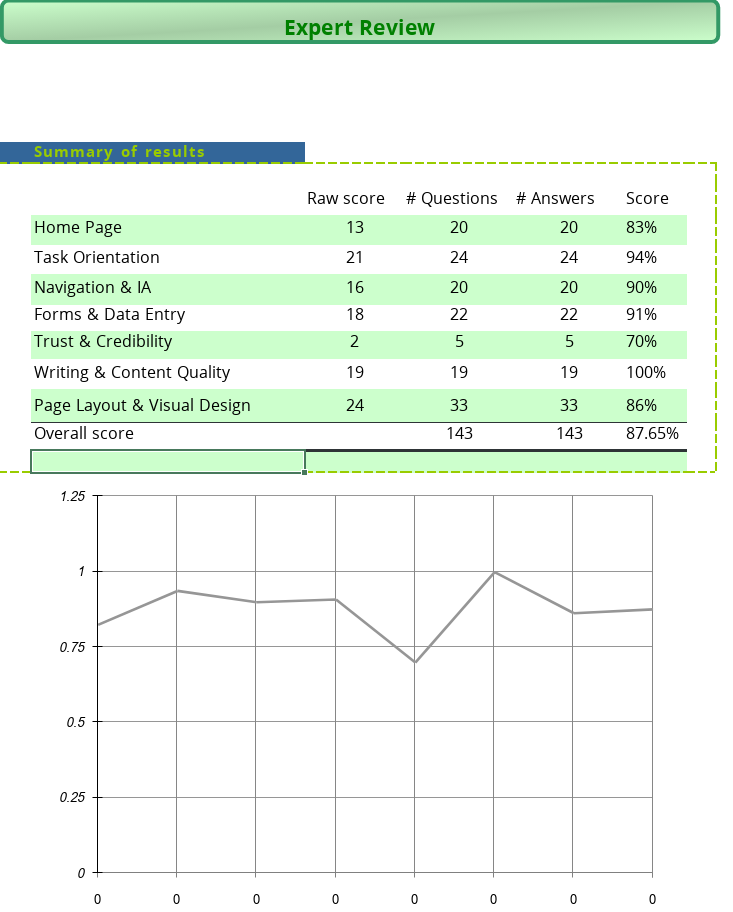
\includegraphics[width=\textwidth]{img/ankieta1}
	\caption{Wyniki ankiety pierwszego eksperta}\label{rys:ankieta1}% Źródło rysunku i etykieta przez którą odwołujemy się do rysunku.
\end{figure}

\begin{figure}
	\centering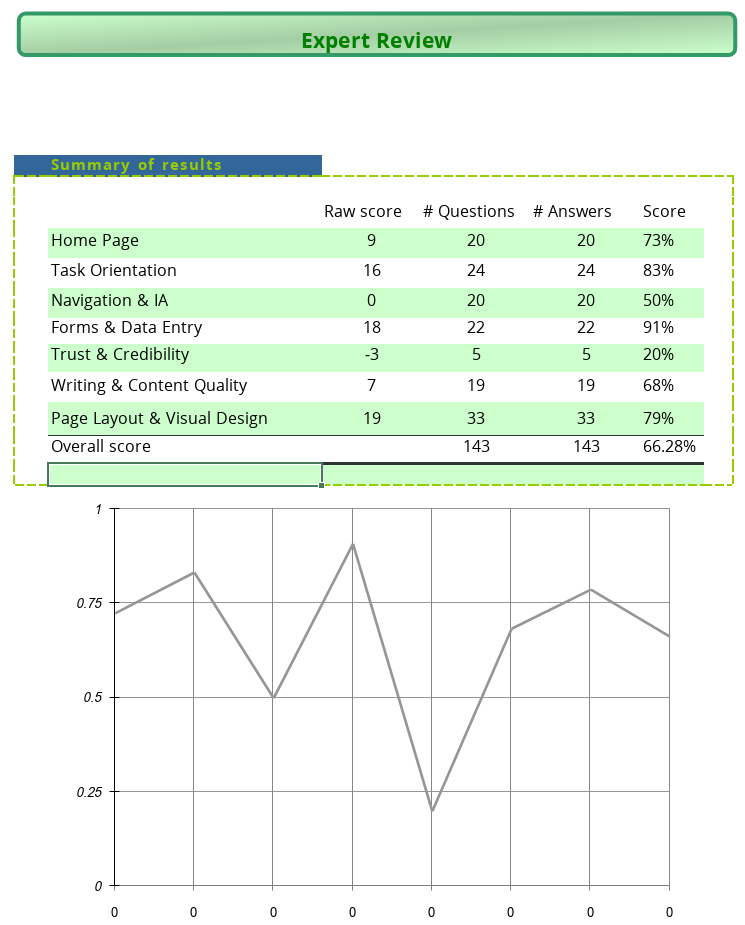
\includegraphics[width=\textwidth]{img/ankieta2}
	\caption{Wyniki ankiety drugiego eksperta}\label{rys:ankieta2}% Źródło rysunku i etykieta przez którą odwołujemy się do rysunku.
\end{figure}

\begin{figure}
	\centering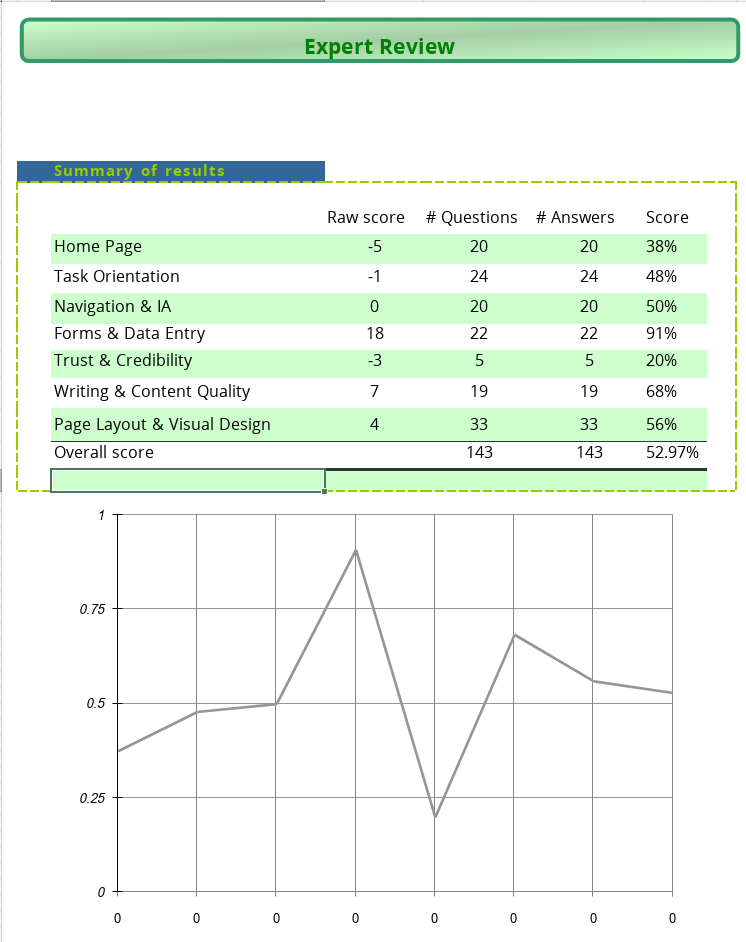
\includegraphics[width=\textwidth]{img/ankieta3}
	\caption{Wyniki ankiety trzeciego eksperta}\label{rys:ankieta3}% Źródło rysunku i etykieta przez którą odwołujemy się do rysunku.
\end{figure}

\begin{figure}
	\centering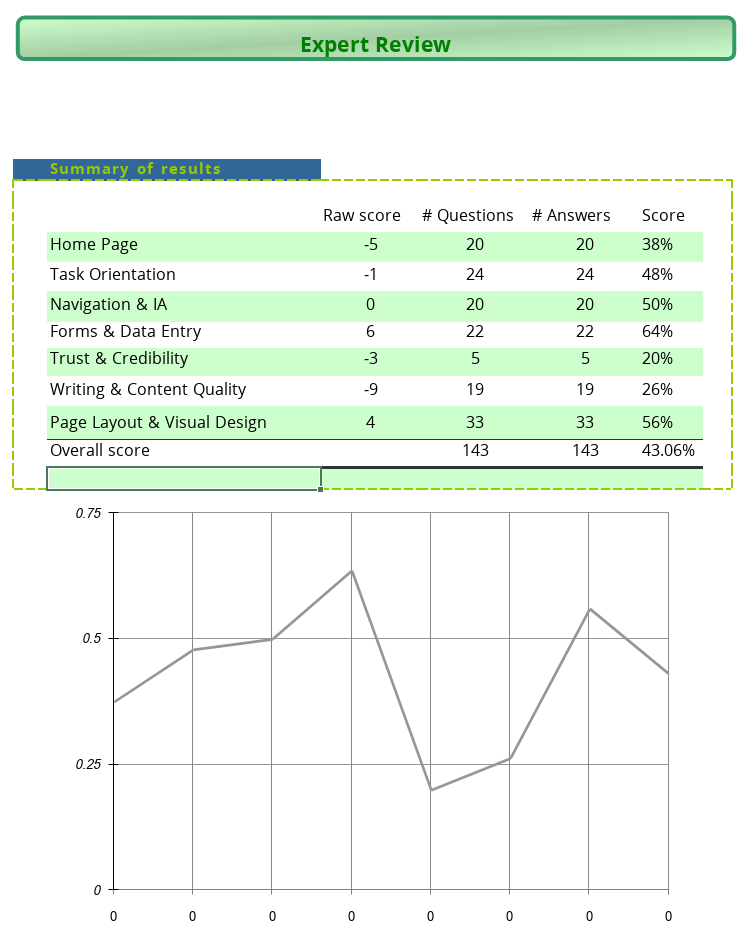
\includegraphics[width=\textwidth]{img/ankieta4}
	\caption{Wyniki ankiety czwartego eksperta}\label{rys:ankieta4}% Źródło rysunku i etykieta przez którą odwołujemy się do rysunku.
\end{figure}

Ten dodatek zawiera wyniki ankiety eksperckiej oceniającej prace,
w której wziął udział czteroosobowy zespół.

Po wynikach ankiet widać, że aplikacja wymaga jeszcze dopracowania.
Problemem jest nawigacja po aplikacji, gdyż wymaga zbyt wielu przejść do ekranów by rozpocząć gre.
Członkowie najchętniej zaczeliby grę, wpisująć w pole tekstowe nazwę repozytorium,
a w drugie odpowiednie filtry by zacząć grę. W aplikacji nie ma też zbyt wielu przydatnych objaśnień.

Według jednego z programistów sam formularz ustawień gry powinien być trochę przeprojektowany,
aby wiadomo było, jakie pola są obowiązkowe, oraz co zmieniają w całej rozgrywce.

Aplikacji przydałby się też odpowiedni dział pomocy, mówiący o tym jak grać w Planning Poker,
oraz jak należy odpowiednio estymować zadania.

Mimo tego aplikacja dzięki swojej integralności z narzędziem Github wyróżnia się na tle konkurencji.
Jeżeli w aplikacji zostanie przeprojektowany sposób tworzenia gry na szybszy
oraz dodanie trochę więcej opcji to może okazać się dość dobrym wyborem dla programistów.

Trzeba jednak przyznać, iż aplikacja spełnia swoje zadanie i z powodzeniem może być wykorzystana
jako narzędzie wspomagające estymację zadań projektowych metodą Planning Poker.


\bibliography{literatura}
\bibliographystyle{dyplom}

\end{document}
